\documentclass[twoside]{book}

% Packages required by doxygen
\usepackage{calc}
\usepackage{doxygen}
\usepackage{graphicx}
\usepackage[utf8]{inputenc}
\usepackage{makeidx}
\usepackage{multicol}
\usepackage{multirow}
\usepackage{textcomp}
\usepackage[table]{xcolor}

% Font selection
\usepackage[T1]{fontenc}
\usepackage{mathptmx}
\usepackage[scaled=.90]{helvet}
\usepackage{courier}
\usepackage{amssymb}
\usepackage{sectsty}
\renewcommand{\familydefault}{\sfdefault}
\allsectionsfont{%
  \fontseries{bc}\selectfont%
  \color{darkgray}%
}
\renewcommand{\DoxyLabelFont}{%
  \fontseries{bc}\selectfont%
  \color{darkgray}%
}

% Page & text layout
\usepackage{geometry}
\geometry{%
  a4paper,%
  top=2.5cm,%
  bottom=2.5cm,%
  left=2.5cm,%
  right=2.5cm%
}
\tolerance=750
\hfuzz=15pt
\hbadness=750
\setlength{\emergencystretch}{15pt}
\setlength{\parindent}{0cm}
\setlength{\parskip}{0.2cm}
\makeatletter
\renewcommand{\paragraph}{%
  \@startsection{paragraph}{4}{0ex}{-1.0ex}{1.0ex}{%
    \normalfont\normalsize\bfseries\SS@parafont%
  }%
}
\renewcommand{\subparagraph}{%
  \@startsection{subparagraph}{5}{0ex}{-1.0ex}{1.0ex}{%
    \normalfont\normalsize\bfseries\SS@subparafont%
  }%
}
\makeatother

% Headers & footers
\usepackage{fancyhdr}
\pagestyle{fancyplain}
\fancyhead[LE]{\fancyplain{}{\bfseries\thepage}}
\fancyhead[CE]{\fancyplain{}{}}
\fancyhead[RE]{\fancyplain{}{\bfseries\leftmark}}
\fancyhead[LO]{\fancyplain{}{\bfseries\rightmark}}
\fancyhead[CO]{\fancyplain{}{}}
\fancyhead[RO]{\fancyplain{}{\bfseries\thepage}}
\fancyfoot[LE]{\fancyplain{}{}}
\fancyfoot[CE]{\fancyplain{}{}}
\fancyfoot[RE]{\fancyplain{}{\bfseries\scriptsize Generated on Sat Dec 26 2015 14\-:07\-:19 for Mari's Tarot by Doxygen }}
\fancyfoot[LO]{\fancyplain{}{\bfseries\scriptsize Generated on Sat Dec 26 2015 14\-:07\-:19 for Mari's Tarot by Doxygen }}
\fancyfoot[CO]{\fancyplain{}{}}
\fancyfoot[RO]{\fancyplain{}{}}
\renewcommand{\footrulewidth}{0.4pt}
\renewcommand{\chaptermark}[1]{%
  \markboth{#1}{}%
}
\renewcommand{\sectionmark}[1]{%
  \markright{\thesection\ #1}%
}

% Indices & bibliography
\usepackage{natbib}
\usepackage[titles]{tocloft}
\setcounter{tocdepth}{3}
\setcounter{secnumdepth}{5}
\makeindex

% Hyperlinks (required, but should be loaded last)
\usepackage{ifpdf}
\ifpdf
  \usepackage[pdftex,pagebackref=true]{hyperref}
\else
  \usepackage[ps2pdf,pagebackref=true]{hyperref}
\fi
\hypersetup{%
  colorlinks=true,%
  linkcolor=blue,%
  citecolor=blue,%
  unicode%
}

% Custom commands
\newcommand{\clearemptydoublepage}{%
  \newpage{\pagestyle{empty}\cleardoublepage}%
}


%===== C O N T E N T S =====

\begin{document}

% Titlepage & ToC
\hypersetup{pageanchor=false}
\pagenumbering{roman}
\begin{titlepage}
\vspace*{7cm}
\begin{center}%
{\Large Mari's Tarot }\\
\vspace*{1cm}
{\large Generated by Doxygen 1.8.6}\\
\vspace*{0.5cm}
{\small Sat Dec 26 2015 14:07:19}\\
\end{center}
\end{titlepage}
\clearemptydoublepage
\tableofcontents
\clearemptydoublepage
\pagenumbering{arabic}
\hypersetup{pageanchor=true}

%--- Begin generated contents ---
\chapter{Hierarchical Index}
\section{\-Class \-Hierarchy}
\-This inheritance list is sorted roughly, but not completely, alphabetically\-:\begin{DoxyCompactList}
\item \contentsline{section}{\-Card}{\pageref{classCard}}{}
\item \contentsline{section}{\-Player\-:\-:card\-Order}{\pageref{structPlayer_1_1cardOrder}}{}
\item \contentsline{section}{\-Deck}{\pageref{classDeck}}{}
\item \contentsline{section}{\-Game}{\pageref{classGame}}{}
\item \contentsline{section}{\-Player}{\pageref{classPlayer}}{}
\begin{DoxyCompactList}
\item \contentsline{section}{\-A\-I}{\pageref{classAI}}{}
\item \contentsline{section}{\-Human}{\pageref{classHuman}}{}
\end{DoxyCompactList}
\item \contentsline{section}{\-Strat\-Diff}{\pageref{classStratDiff}}{}
\begin{DoxyCompactList}
\item \contentsline{section}{\-Beginner}{\pageref{classBeginner}}{}
\end{DoxyCompactList}
\item \contentsline{section}{\-Strat\-Lang}{\pageref{classStratLang}}{}
\item \contentsline{section}{\-Team}{\pageref{classTeam}}{}
\item \contentsline{section}{\-Trick}{\pageref{classTrick}}{}
\end{DoxyCompactList}

\chapter{Class Index}
\section{Class List}
Here are the classes, structs, unions and interfaces with brief descriptions\-:\begin{DoxyCompactList}
\item\contentsline{section}{\hyperlink{classAI}{A\-I} \\*This class defines \hyperlink{classAI}{A\-I} players }{\pageref{classAI}}{}
\item\contentsline{section}{\hyperlink{classBeginner}{Beginner} \\*One of the proposed difficulty }{\pageref{classBeginner}}{}
\item\contentsline{section}{\hyperlink{classCard}{Card} \\*\hyperlink{classCard}{Card} is the class compiling all useful information on cards\-: points, suit, value.. }{\pageref{classCard}}{}
\item\contentsline{section}{\hyperlink{structPlayer_1_1cardOrder}{Player\-::card\-Order} \\*A structure to automatically fix an insert order into cards' sets }{\pageref{structPlayer_1_1cardOrder}}{}
\item\contentsline{section}{\hyperlink{classDeck}{Deck} \\*\hyperlink{classDeck}{Deck} is the class managing the deck of cards. Used as well as for the game deck, but also for a counting cards \hyperlink{classAI}{A\-I} }{\pageref{classDeck}}{}
\item\contentsline{section}{\hyperlink{classGame}{Game} \\*\hyperlink{classGame}{Game} is one of the main class of Tarot. Here are defined rules, games' turns, scores, etc }{\pageref{classGame}}{}
\item\contentsline{section}{\hyperlink{classHuman}{Human} \\*\hyperlink{classHuman}{Human} is the class implementing \hyperlink{classHuman}{Human} player actions, like playing a card }{\pageref{classHuman}}{}
\item\contentsline{section}{\hyperlink{classPlayer}{Player} \\*\hyperlink{classPlayer}{Player} is an abstract class presenting a common interface for \hyperlink{classAI}{A\-I} and \hyperlink{classHuman}{Human} players }{\pageref{classPlayer}}{}
\item\contentsline{section}{\hyperlink{classStratDiff}{Strat\-Diff} \\*\hyperlink{classStratDiff}{Strat\-Diff} is the abstract class handling the Strategy pattern for applying different \hyperlink{classAI}{A\-I} difficulties }{\pageref{classStratDiff}}{}
\item\contentsline{section}{\hyperlink{classStratLang}{Strat\-Lang} \\*\hyperlink{classStratDiff}{Strat\-Diff} is the abstract class handling the Strategy pattern to propose different languages }{\pageref{classStratLang}}{}
\item\contentsline{section}{\hyperlink{classTeam}{Team} \\*\hyperlink{classTeam}{Team} is the class handling team management }{\pageref{classTeam}}{}
\item\contentsline{section}{\hyperlink{classTrick}{Trick} \\*This class manages the current and previously played tricks }{\pageref{classTrick}}{}
\end{DoxyCompactList}

\chapter{Class Documentation}
\hypertarget{classAI}{\section{A\-I Class Reference}
\label{classAI}\index{A\-I@{A\-I}}
}


This class defines \hyperlink{classAI}{A\-I} players.  




{\ttfamily \#include $<$A\-I.\-hpp$>$}

Inheritance diagram for A\-I\-:\begin{figure}[H]
\begin{center}
\leavevmode
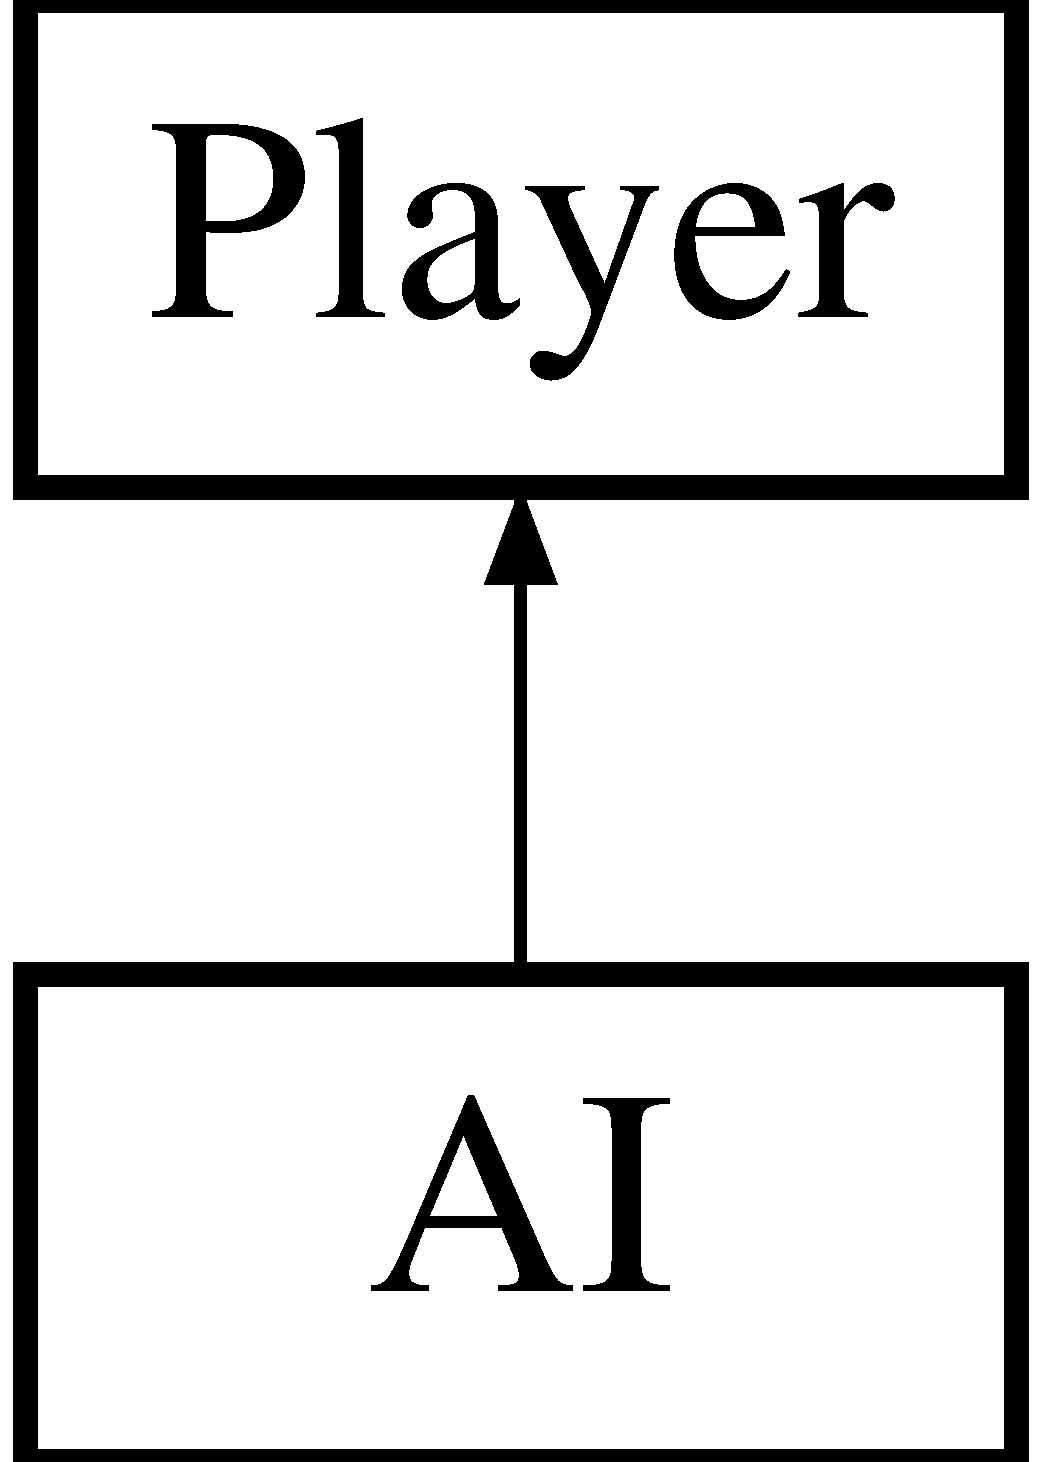
\includegraphics[height=2.000000cm]{classAI}
\end{center}
\end{figure}
\subsection*{Public Member Functions}
\begin{DoxyCompactItemize}
\item 
\hyperlink{classAI_a059fcf3ea09f908bca75567937f7e8a7}{A\-I} (const string \&\hyperlink{classPlayer_acf0355128a99ee20ad9931b760fb2de1}{name}, const vector$<$ string $>$ \&known\-Partners)
\begin{DoxyCompactList}\small\item\em \hyperlink{classAI}{A\-I} constructor. \end{DoxyCompactList}\item 
bool \hyperlink{classAI_aec78eb8010bdcd99c899aaa7af79d9ea}{is\-Opponent} (const string \&\hyperlink{classPlayer_acf0355128a99ee20ad9931b760fb2de1}{name}) const 
\begin{DoxyCompactList}\small\item\em To know if someone is your opponent. \end{DoxyCompactList}\item 
bool \hyperlink{classAI_a0cd8c8e4a646c6c1ae51c7812eb1194e}{is\-Partner} (const string \&\hyperlink{classPlayer_acf0355128a99ee20ad9931b760fb2de1}{name}) const 
\begin{DoxyCompactList}\small\item\em To know if someone is your partner. \end{DoxyCompactList}\item 
bool \hyperlink{classAI_a01cd7c1760412dde024605226591328c}{have\-Suit} (const string \&\hyperlink{classPlayer_acf0355128a99ee20ad9931b760fb2de1}{name}, const Suits suit) const 
\begin{DoxyCompactList}\small\item\em Given a \hyperlink{classPlayer}{Player} p, does p have at least one card on the asked suit? \end{DoxyCompactList}\item 
bool \hyperlink{classAI_affad35d086fe81539b07a5626b19c1bb}{opponents\-Have\-Suit} (const Suits suit) const 
\begin{DoxyCompactList}\small\item\em Do opponents have at least one card on the asked suit? \end{DoxyCompactList}\item 
shared\-\_\-ptr$<$ \hyperlink{classCard}{Card} $>$ \hyperlink{classAI_a3f5b2888e03634db701c66f82a4f03a8}{play\-Card} (shared\-\_\-ptr$<$ \hyperlink{classCard}{Card} $>$ reference\-Card, shared\-\_\-ptr$<$ \hyperlink{classCard}{Card} $>$ high\-Trump)
\begin{DoxyCompactList}\small\item\em Choose what card one plays, given the first card and the highest trump of the trick. \end{DoxyCompactList}\item 
void \hyperlink{classAI_a6cda26d3bf7238b1a7ea3725bf4aabb7}{new\-Game} ()
\begin{DoxyCompactList}\small\item\em Must be called when starting a new game. \end{DoxyCompactList}\item 
Biddings \hyperlink{classAI_a9e2fd7ff440ada8339135c23b73e1a96}{bid} (const Biddings best\-Bid, const bool chelem\-Announced) const 
\begin{DoxyCompactList}\small\item\em Called to decide if one proposes a bid or not, and if any, what bid. \end{DoxyCompactList}\item 
set$<$ shared\-\_\-ptr$<$ \hyperlink{classCard}{Card} $>$ $>$ \hyperlink{classAI_ad12a3efd1da4acc6e1855bd7262779e3}{make\-Ecart} (const int dog\-Size)
\begin{DoxyCompactList}\small\item\em To make the ecart once one takes the dog. \end{DoxyCompactList}\item 
void \hyperlink{classAI_a19cae044bb7f221819f61b017b6a7ffe}{set\-Difficulty} (shared\-\_\-ptr$<$ \hyperlink{classStratDiff}{Strat\-Diff} $>$ diff)
\begin{DoxyCompactList}\small\item\em Inline function to set the difficulty (set a Strategy concrete class). \end{DoxyCompactList}\end{DoxyCompactItemize}
\subsection*{Additional Inherited Members}


\subsection{Detailed Description}
This class defines \hyperlink{classAI}{A\-I} players. 

The class \hyperlink{classAI}{A\-I} extends \hyperlink{classPlayer}{Player} and shows an interface for actions like play\-Card, make a bid, etc. Actions' implementation is decoupled from the class with a Strategy pattern, where concret classes correspond to a level of difficulty. 

\subsection{Constructor \& Destructor Documentation}
\hypertarget{classAI_a059fcf3ea09f908bca75567937f7e8a7}{\index{A\-I@{A\-I}!A\-I@{A\-I}}
\index{A\-I@{A\-I}!AI@{A\-I}}
\subsubsection[{A\-I}]{\setlength{\rightskip}{0pt plus 5cm}A\-I\-::\-A\-I (
\begin{DoxyParamCaption}
\item[{const string \&}]{name, }
\item[{const vector$<$ string $>$ \&}]{known\-Partners}
\end{DoxyParamCaption}
)}}\label{classAI_a059fcf3ea09f908bca75567937f7e8a7}


\hyperlink{classAI}{A\-I} constructor. 


\begin{DoxyParams}{Parameters}
{\em name} & A string for the \hyperlink{classAI}{A\-I} name. \\
\hline
{\em known\-Partners} & A vector of strings composed of the name of its partners. \\
\hline
\end{DoxyParams}


\subsection{Member Function Documentation}
\hypertarget{classAI_a9e2fd7ff440ada8339135c23b73e1a96}{\index{A\-I@{A\-I}!bid@{bid}}
\index{bid@{bid}!AI@{A\-I}}
\subsubsection[{bid}]{\setlength{\rightskip}{0pt plus 5cm}Biddings A\-I\-::bid (
\begin{DoxyParamCaption}
\item[{const Biddings}]{best\-Bid, }
\item[{const bool}]{chelem\-Announced}
\end{DoxyParamCaption}
) const\hspace{0.3cm}{\ttfamily [virtual]}}}\label{classAI_a9e2fd7ff440ada8339135c23b73e1a96}


Called to decide if one proposes a bid or not, and if any, what bid. 

bid is delegated to the difficulty Strategy. 
\begin{DoxyParams}{Parameters}
{\em best\-Bid} & The best bid proposed so far. \\
\hline
{\em chelem\-Announced} & A Boolean to know if someone has declared a chelem. \\
\hline
\end{DoxyParams}
\begin{DoxyReturn}{Returns}
Our bid (Biddings\-::none if one passes). 
\end{DoxyReturn}


Implements \hyperlink{classPlayer_a4bb658ca7b46f32a42578b884ad7fe82}{Player}.

\hypertarget{classAI_a01cd7c1760412dde024605226591328c}{\index{A\-I@{A\-I}!have\-Suit@{have\-Suit}}
\index{have\-Suit@{have\-Suit}!AI@{A\-I}}
\subsubsection[{have\-Suit}]{\setlength{\rightskip}{0pt plus 5cm}bool A\-I\-::have\-Suit (
\begin{DoxyParamCaption}
\item[{const string \&}]{name, }
\item[{const Suits}]{suit}
\end{DoxyParamCaption}
) const}}\label{classAI_a01cd7c1760412dde024605226591328c}


Given a \hyperlink{classPlayer}{Player} p, does p have at least one card on the asked suit? 


\begin{DoxyParams}{Parameters}
{\em name} & The \hyperlink{classPlayer}{Player}'s name in string. \\
\hline
{\em suit} & The asked suit. \\
\hline
\end{DoxyParams}
\begin{DoxyReturn}{Returns}
False iff one is sure p does not have any cards of the asked suit. 
\end{DoxyReturn}
\hypertarget{classAI_aec78eb8010bdcd99c899aaa7af79d9ea}{\index{A\-I@{A\-I}!is\-Opponent@{is\-Opponent}}
\index{is\-Opponent@{is\-Opponent}!AI@{A\-I}}
\subsubsection[{is\-Opponent}]{\setlength{\rightskip}{0pt plus 5cm}bool A\-I\-::is\-Opponent (
\begin{DoxyParamCaption}
\item[{const string \&}]{name}
\end{DoxyParamCaption}
) const\hspace{0.3cm}{\ttfamily [inline]}}}\label{classAI_aec78eb8010bdcd99c899aaa7af79d9ea}


To know if someone is your opponent. 


\begin{DoxyParams}{Parameters}
{\em name} & The \hyperlink{classPlayer}{Player}'s name in string. \\
\hline
\end{DoxyParams}
\begin{DoxyReturn}{Returns}
If the given \hyperlink{classPlayer}{Player} is an opponent or not. 
\end{DoxyReturn}
\hypertarget{classAI_a0cd8c8e4a646c6c1ae51c7812eb1194e}{\index{A\-I@{A\-I}!is\-Partner@{is\-Partner}}
\index{is\-Partner@{is\-Partner}!AI@{A\-I}}
\subsubsection[{is\-Partner}]{\setlength{\rightskip}{0pt plus 5cm}bool A\-I\-::is\-Partner (
\begin{DoxyParamCaption}
\item[{const string \&}]{name}
\end{DoxyParamCaption}
) const\hspace{0.3cm}{\ttfamily [inline]}}}\label{classAI_a0cd8c8e4a646c6c1ae51c7812eb1194e}


To know if someone is your partner. 


\begin{DoxyParams}{Parameters}
{\em name} & The \hyperlink{classPlayer}{Player}'s name in string. \\
\hline
\end{DoxyParams}
\begin{DoxyReturn}{Returns}
If the given \hyperlink{classPlayer}{Player} is an partner or not. 
\end{DoxyReturn}
\hypertarget{classAI_ad12a3efd1da4acc6e1855bd7262779e3}{\index{A\-I@{A\-I}!make\-Ecart@{make\-Ecart}}
\index{make\-Ecart@{make\-Ecart}!AI@{A\-I}}
\subsubsection[{make\-Ecart}]{\setlength{\rightskip}{0pt plus 5cm}set$<$ shared\-\_\-ptr$<$ {\bf Card} $>$ $>$ A\-I\-::make\-Ecart (
\begin{DoxyParamCaption}
\item[{const int}]{dog\-Size}
\end{DoxyParamCaption}
)\hspace{0.3cm}{\ttfamily [virtual]}}}\label{classAI_ad12a3efd1da4acc6e1855bd7262779e3}


To make the ecart once one takes the dog. 

make\-Ecart is delegated to the difficulty Strategy. 
\begin{DoxyParams}{Parameters}
{\em dog\-Size} & The number of card one must include into the ecart. \\
\hline
\end{DoxyParams}
\begin{DoxyReturn}{Returns}
A set of \hyperlink{classCard}{Card} pointers for the cards one places into the ecart. 
\end{DoxyReturn}


Implements \hyperlink{classPlayer_a34c9e9f402c6a68d6e16caebdb93a33f}{Player}.

\hypertarget{classAI_a6cda26d3bf7238b1a7ea3725bf4aabb7}{\index{A\-I@{A\-I}!new\-Game@{new\-Game}}
\index{new\-Game@{new\-Game}!AI@{A\-I}}
\subsubsection[{new\-Game}]{\setlength{\rightskip}{0pt plus 5cm}void A\-I\-::new\-Game (
\begin{DoxyParamCaption}
{}
\end{DoxyParamCaption}
)\hspace{0.3cm}{\ttfamily [virtual]}}}\label{classAI_a6cda26d3bf7238b1a7ea3725bf4aabb7}


Must be called when starting a new game. 

Flush to zero some variables and pointers. 

Implements \hyperlink{classPlayer_a76a707ceb6f24b0a2a801434ee5a60ad}{Player}.

\hypertarget{classAI_affad35d086fe81539b07a5626b19c1bb}{\index{A\-I@{A\-I}!opponents\-Have\-Suit@{opponents\-Have\-Suit}}
\index{opponents\-Have\-Suit@{opponents\-Have\-Suit}!AI@{A\-I}}
\subsubsection[{opponents\-Have\-Suit}]{\setlength{\rightskip}{0pt plus 5cm}bool A\-I\-::opponents\-Have\-Suit (
\begin{DoxyParamCaption}
\item[{const Suits}]{suit}
\end{DoxyParamCaption}
) const}}\label{classAI_affad35d086fe81539b07a5626b19c1bb}


Do opponents have at least one card on the asked suit? 


\begin{DoxyParams}{Parameters}
{\em suit} & The asked suit. \\
\hline
\end{DoxyParams}
\begin{DoxyReturn}{Returns}
False iff one is sure no opponent player has a card of the asked suit. 
\end{DoxyReturn}
\hypertarget{classAI_a3f5b2888e03634db701c66f82a4f03a8}{\index{A\-I@{A\-I}!play\-Card@{play\-Card}}
\index{play\-Card@{play\-Card}!AI@{A\-I}}
\subsubsection[{play\-Card}]{\setlength{\rightskip}{0pt plus 5cm}shared\-\_\-ptr$<$ {\bf Card} $>$ A\-I\-::play\-Card (
\begin{DoxyParamCaption}
\item[{shared\-\_\-ptr$<$ {\bf Card} $>$}]{reference\-Card, }
\item[{shared\-\_\-ptr$<$ {\bf Card} $>$}]{high\-Trump}
\end{DoxyParamCaption}
)\hspace{0.3cm}{\ttfamily [virtual]}}}\label{classAI_a3f5b2888e03634db701c66f82a4f03a8}


Choose what card one plays, given the first card and the highest trump of the trick. 

play\-Card is delegated to the difficulty Strategy. 
\begin{DoxyParams}{Parameters}
{\em reference\-Card} & A \hyperlink{classCard}{Card} pointer of the first played card of the trick. \\
\hline
{\em high\-Trump} & A \hyperlink{classCard}{Card} pointer of the highest trump of the trick. \\
\hline
\end{DoxyParams}
\begin{DoxyReturn}{Returns}
The card the \hyperlink{classAI}{A\-I} plays. 
\end{DoxyReturn}


Implements \hyperlink{classPlayer_aeba090a124bfd9a3666d2d793439cae0}{Player}.

\hypertarget{classAI_a19cae044bb7f221819f61b017b6a7ffe}{\index{A\-I@{A\-I}!set\-Difficulty@{set\-Difficulty}}
\index{set\-Difficulty@{set\-Difficulty}!AI@{A\-I}}
\subsubsection[{set\-Difficulty}]{\setlength{\rightskip}{0pt plus 5cm}void A\-I\-::set\-Difficulty (
\begin{DoxyParamCaption}
\item[{shared\-\_\-ptr$<$ {\bf Strat\-Diff} $>$}]{diff}
\end{DoxyParamCaption}
)\hspace{0.3cm}{\ttfamily [inline]}}}\label{classAI_a19cae044bb7f221819f61b017b6a7ffe}


Inline function to set the difficulty (set a Strategy concrete class). 


\begin{DoxyParams}{Parameters}
{\em diff} & A pointer on the difficulty to set. \\
\hline
\end{DoxyParams}


The documentation for this class was generated from the following files\-:\begin{DoxyCompactItemize}
\item 
src/A\-I.\-hpp\item 
src/A\-I.\-cpp\end{DoxyCompactItemize}

\hypertarget{classBeginner}{\section{\-Beginner \-Class \-Reference}
\label{classBeginner}\index{\-Beginner@{\-Beginner}}
}


\-One of the proposed difficulty.  




{\ttfamily \#include $<$\-Beginner.\-hpp$>$}

\-Inheritance diagram for \-Beginner\-:\begin{figure}[H]
\begin{center}
\leavevmode
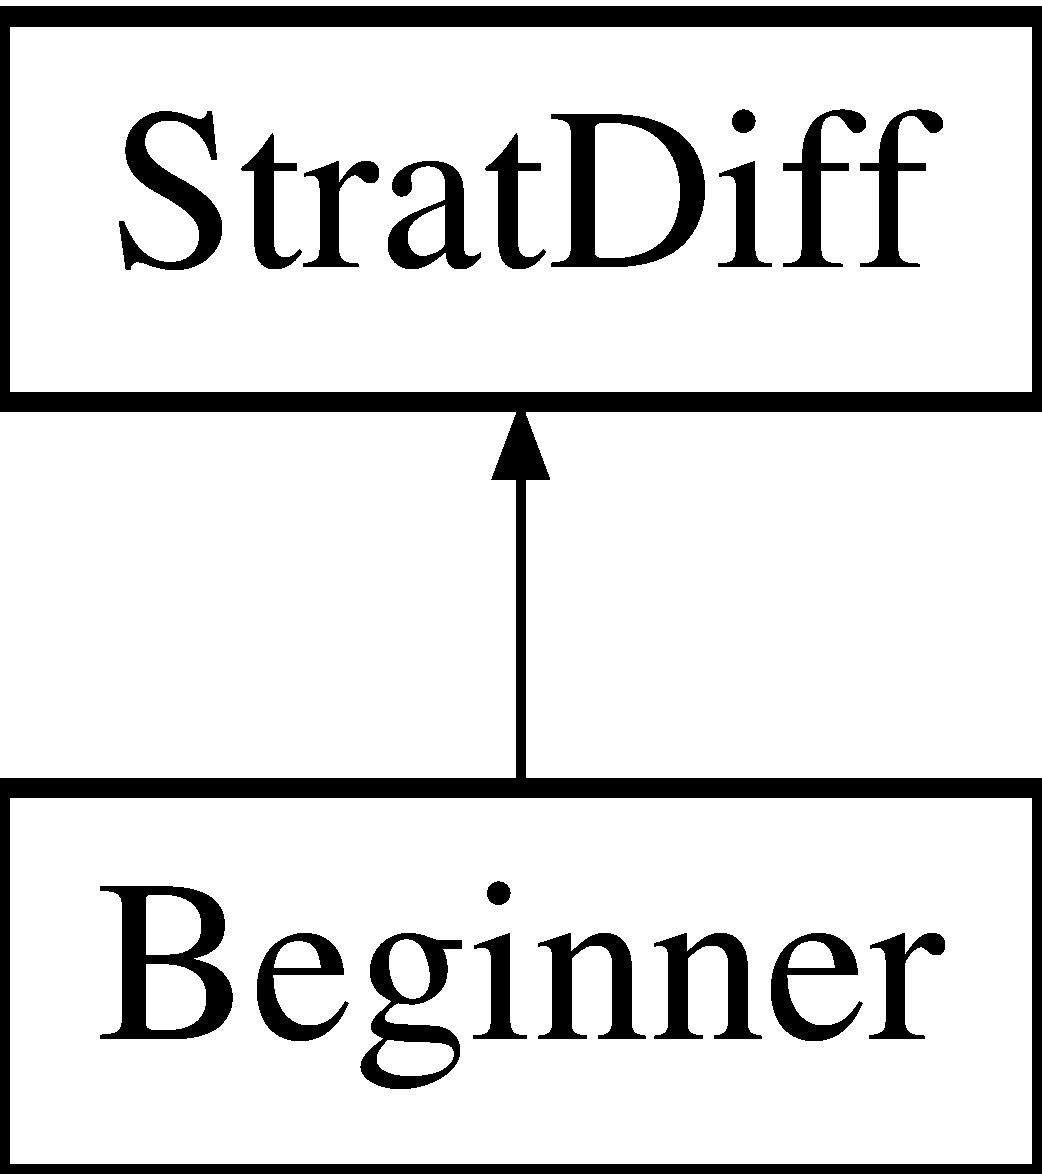
\includegraphics[height=2.000000cm]{classBeginner}
\end{center}
\end{figure}
\subsection*{\-Public \-Member \-Functions}
\begin{DoxyCompactItemize}
\item 
shared\-\_\-ptr$<$ \hyperlink{classCard}{\-Card} $>$ \hyperlink{classBeginner_a73e2bf8d807166c994c42fd3b6bfc7bf}{play\-Card} (const vector$<$ shared\-\_\-ptr$<$ \hyperlink{classCard}{\-Card} $>$ $>$ \&cards\-Can\-Play) const 
\begin{DoxyCompactList}\small\item\em \-Choose what card we play, given the first card and the highest trump of the trick. \end{DoxyCompactList}\item 
\-Biddings \hyperlink{classBeginner_ad051797028f352b16df271fb24c435f6}{bid} (const \-Biddings best\-Bid, const int number\-Oudlers, const bool chelem\-Announced) const 
\begin{DoxyCompactList}\small\item\em \-Called to decide if we propose a bid or not, and if any, what bid. \end{DoxyCompactList}\item 
set$<$ shared\-\_\-ptr$<$ \hyperlink{classCard}{\-Card} $>$ $>$ \hyperlink{classBeginner_a7817d38e018ac5e1d9dbb42923ef0752}{make\-Ecart} (const int dog\-Size, const vector$<$ shared\-\_\-ptr$<$ \hyperlink{classCard}{\-Card} $>$ $>$ \&all\-Cards) const 
\begin{DoxyCompactList}\small\item\em \-To make the ecart once we take the dog. \end{DoxyCompactList}\end{DoxyCompactItemize}


\subsection{\-Detailed \-Description}
\-One of the proposed difficulty. 

\hyperlink{classBeginner}{\-Beginner} is one of the concrete class of the \-Strategy pattern dealing with the game difficulty (i.\-e., how good the \hyperlink{classAI}{\-A\-I} is). 

\subsection{\-Member \-Function \-Documentation}
\hypertarget{classBeginner_ad051797028f352b16df271fb24c435f6}{\index{\-Beginner@{\-Beginner}!bid@{bid}}
\index{bid@{bid}!Beginner@{\-Beginner}}
\subsubsection[{bid}]{\setlength{\rightskip}{0pt plus 5cm}\-Biddings {\bf \-Beginner\-::bid} (
\begin{DoxyParamCaption}
\item[{const \-Biddings}]{best\-Bid, }
\item[{const int}]{number\-Oudlers, }
\item[{const bool}]{chelem\-Announced}
\end{DoxyParamCaption}
) const\hspace{0.3cm}{\ttfamily  \mbox{[}virtual\mbox{]}}}}\label{classBeginner_ad051797028f352b16df271fb24c435f6}


\-Called to decide if we propose a bid or not, and if any, what bid. 

bid is delegated to the difficulty \-Strategy. 
\begin{DoxyParams}{\-Parameters}
{\em best\-Bid} & \-The best bid proposed so far. \\
\hline
{\em number\-Oudlers} & \-The number of oudlers we have in our hand. \\
\hline
{\em chelem\-Announced} & \-A \-Boolean to know if someone has declared a chelem. \\
\hline
\end{DoxyParams}
\begin{DoxyReturn}{\-Returns}
\-Our bid (\-Biddings\-::none if we pass). 
\end{DoxyReturn}


\-Implements \hyperlink{classStratDiff_ac77eac57b96c445edeb36c7205cfbcf4}{\-Strat\-Diff}.

\hypertarget{classBeginner_a7817d38e018ac5e1d9dbb42923ef0752}{\index{\-Beginner@{\-Beginner}!make\-Ecart@{make\-Ecart}}
\index{make\-Ecart@{make\-Ecart}!Beginner@{\-Beginner}}
\subsubsection[{make\-Ecart}]{\setlength{\rightskip}{0pt plus 5cm}set$<$ shared\-\_\-ptr$<$ {\bf \-Card} $>$ $>$ {\bf \-Beginner\-::make\-Ecart} (
\begin{DoxyParamCaption}
\item[{const int}]{dog\-Size, }
\item[{const vector$<$ shared\-\_\-ptr$<$ {\bf \-Card} $>$ $>$ \&}]{all\-Cards}
\end{DoxyParamCaption}
) const\hspace{0.3cm}{\ttfamily  \mbox{[}virtual\mbox{]}}}}\label{classBeginner_a7817d38e018ac5e1d9dbb42923ef0752}


\-To make the ecart once we take the dog. 

make\-Ecart is delegated to the difficulty \-Strategy. 
\begin{DoxyParams}{\-Parameters}
{\em dog\-Size} & \-The number of card we must include into the ecart. \\
\hline
{\em all\-Cards} & \-The vector of all our cards, including the dog. \\
\hline
\end{DoxyParams}
\begin{DoxyReturn}{\-Returns}
\-A set of \hyperlink{classCard}{\-Card} pointers for the cards we place into the ecart. 
\end{DoxyReturn}


\-Implements \hyperlink{classStratDiff_a892386aed17049a0d757170603fddce1}{\-Strat\-Diff}.

\hypertarget{classBeginner_a73e2bf8d807166c994c42fd3b6bfc7bf}{\index{\-Beginner@{\-Beginner}!play\-Card@{play\-Card}}
\index{play\-Card@{play\-Card}!Beginner@{\-Beginner}}
\subsubsection[{play\-Card}]{\setlength{\rightskip}{0pt plus 5cm}shared\-\_\-ptr$<$ {\bf \-Card} $>$ {\bf \-Beginner\-::play\-Card} (
\begin{DoxyParamCaption}
\item[{const vector$<$ shared\-\_\-ptr$<$ {\bf \-Card} $>$ $>$ \&}]{cards\-Can\-Play}
\end{DoxyParamCaption}
) const\hspace{0.3cm}{\ttfamily  \mbox{[}virtual\mbox{]}}}}\label{classBeginner_a73e2bf8d807166c994c42fd3b6bfc7bf}


\-Choose what card we play, given the first card and the highest trump of the trick. 


\begin{DoxyParams}{\-Parameters}
{\em card\-Can\-Play} & \-The vector of cards one is allowed to play. \\
\hline
\end{DoxyParams}
\begin{DoxyReturn}{\-Returns}
\-The card we play. 
\end{DoxyReturn}


\-Implements \hyperlink{classStratDiff_a550903bf95e6a897f346debab972f33a}{\-Strat\-Diff}.



\-The documentation for this class was generated from the following files\-:\begin{DoxyCompactItemize}
\item 
include/\-Beginner.\-hpp\item 
src/\-Beginner.\-cpp\end{DoxyCompactItemize}

\hypertarget{classCard}{\section{\-Card \-Class \-Reference}
\label{classCard}\index{\-Card@{\-Card}}
}


\hyperlink{classCard}{\-Card} is the class compiling all useful information on cards\-: points, suit, value...  




{\ttfamily \#include $<$\-Card.\-hpp$>$}

\subsection*{\-Public \-Member \-Functions}
\begin{DoxyCompactItemize}
\item 
\hyperlink{classCard_a113a46b46e64efe0fd98a42df301db9a}{\-Card} (const \-Suits suit, const int value, const double points, const bool oudler)
\begin{DoxyCompactList}\small\item\em \-The unique constructor for \hyperlink{classCard}{\-Card}. \end{DoxyCompactList}\item 
\hypertarget{classCard_adf11e6396788e2e832d3bdf29880593f}{double \hyperlink{classCard_adf11e6396788e2e832d3bdf29880593f}{get\-Points} () const }\label{classCard_adf11e6396788e2e832d3bdf29880593f}

\begin{DoxyCompactList}\small\item\em \-Inline assessor to get the card's points. \end{DoxyCompactList}\item 
\hypertarget{classCard_a77f39ecaee335e62e267e44e07a15ebe}{\-Suits \hyperlink{classCard_a77f39ecaee335e62e267e44e07a15ebe}{get\-Suit} () const }\label{classCard_a77f39ecaee335e62e267e44e07a15ebe}

\begin{DoxyCompactList}\small\item\em \-Inline assessor to get the card's suit. \end{DoxyCompactList}\item 
\hypertarget{classCard_ab70c98dd7bfc44f87c5914990737e79d}{int \hyperlink{classCard_ab70c98dd7bfc44f87c5914990737e79d}{get\-Value} () const }\label{classCard_ab70c98dd7bfc44f87c5914990737e79d}

\begin{DoxyCompactList}\small\item\em \-Inline assessor to get the card's value. \end{DoxyCompactList}\item 
\hypertarget{classCard_aa05732992ee8352a205a15d89f4edda4}{bool \hyperlink{classCard_aa05732992ee8352a205a15d89f4edda4}{is\-Fool} () const }\label{classCard_aa05732992ee8352a205a15d89f4edda4}

\begin{DoxyCompactList}\small\item\em \-Inline function returning true iif the card is the \-Fool. \end{DoxyCompactList}\item 
\hypertarget{classCard_ad9674d010674d0a536994147696abc6d}{bool \hyperlink{classCard_ad9674d010674d0a536994147696abc6d}{is\-Trump} () const }\label{classCard_ad9674d010674d0a536994147696abc6d}

\begin{DoxyCompactList}\small\item\em \-Inline function returning true iif the card is a trump. \end{DoxyCompactList}\item 
\hypertarget{classCard_a8ac4b04ac18721afdff8d504a7621a97}{bool \hyperlink{classCard_a8ac4b04ac18721afdff8d504a7621a97}{is\-Oudler} () const }\label{classCard_a8ac4b04ac18721afdff8d504a7621a97}

\begin{DoxyCompactList}\small\item\em \-Inline function returning true iif the card is an oudler. \end{DoxyCompactList}\item 
\hypertarget{classCard_ac8978fa4de9e59246381ebd2f9c5ecfc}{bool \hyperlink{classCard_ac8978fa4de9e59246381ebd2f9c5ecfc}{is\-Face\-Card} () const }\label{classCard_ac8978fa4de9e59246381ebd2f9c5ecfc}

\begin{DoxyCompactList}\small\item\em \-Inline function returning true iif the card is a face card. \end{DoxyCompactList}\item 
bool \hyperlink{classCard_a50bd8a1a5d5bdfce5727718844f87ce8}{operator$>$} (const \hyperlink{classCard}{\-Card} \&card) const 
\begin{DoxyCompactList}\small\item\em \-A greater-\/than comparator to make easier the comparison between cards. \end{DoxyCompactList}\item 
bool \hyperlink{classCard_a0210e809d9ec749824716ec1f5ebbf8a}{operator$<$} (const \hyperlink{classCard}{\-Card} \&card) const 
\begin{DoxyCompactList}\small\item\em \-A less-\/than comparator to make easier the comparison between cards. \end{DoxyCompactList}\item 
bool \hyperlink{classCard_a54a1553ca40e32768ee09465447b8090}{operator==} (const \hyperlink{classCard}{\-Card} \&card) const 
\begin{DoxyCompactList}\small\item\em \-An equal comparator to make easier the comparison between cards. \end{DoxyCompactList}\item 
bool \hyperlink{classCard_a2c531d32de5e76e758254b9d03689ae5}{is\-Comparable} (const \hyperlink{classCard}{\-Card} \&card) const 
\begin{DoxyCompactList}\small\item\em \-A function to decide if two cards are comparable. \end{DoxyCompactList}\end{DoxyCompactItemize}
\subsection*{\-Friends}
\begin{DoxyCompactItemize}
\item 
\hypertarget{classCard_a19eb35e24a8f6368e34575698fca9008}{ostream \& \hyperlink{classCard_a19eb35e24a8f6368e34575698fca9008}{operator$<$$<$} (ostream \&, const \hyperlink{classCard}{\-Card} \&)}\label{classCard_a19eb35e24a8f6368e34575698fca9008}

\begin{DoxyCompactList}\small\item\em \-Surcharging $<$$<$ to make std\-::cout easier. \end{DoxyCompactList}\end{DoxyCompactItemize}


\subsection{\-Detailed \-Description}
\hyperlink{classCard}{\-Card} is the class compiling all useful information on cards\-: points, suit, value... 

\subsection{\-Constructor \& \-Destructor \-Documentation}
\hypertarget{classCard_a113a46b46e64efe0fd98a42df301db9a}{\index{\-Card@{\-Card}!\-Card@{\-Card}}
\index{\-Card@{\-Card}!Card@{\-Card}}
\subsubsection[{\-Card}]{\setlength{\rightskip}{0pt plus 5cm}{\bf \-Card\-::\-Card} (
\begin{DoxyParamCaption}
\item[{const \-Suits}]{suit, }
\item[{const int}]{value, }
\item[{const double}]{points, }
\item[{const bool}]{oudler}
\end{DoxyParamCaption}
)}}\label{classCard_a113a46b46e64efe0fd98a42df301db9a}


\-The unique constructor for \hyperlink{classCard}{\-Card}. 


\begin{DoxyParams}{\-Parameters}
{\em suit} & \-The card's suit. \\
\hline
{\em value} & \-Its value (11, 12, 13 and 14 for a \-Jack, \-Knigh, \-Queen and \-King, respectively). \\
\hline
{\em points} & \-Its points, needing a real value. \\
\hline
{\em oudler} & \-A \-Boolean set to true iff the card is an oudler. \\
\hline
\end{DoxyParams}


\subsection{\-Member \-Function \-Documentation}
\hypertarget{classCard_a2c531d32de5e76e758254b9d03689ae5}{\index{\-Card@{\-Card}!is\-Comparable@{is\-Comparable}}
\index{is\-Comparable@{is\-Comparable}!Card@{\-Card}}
\subsubsection[{is\-Comparable}]{\setlength{\rightskip}{0pt plus 5cm}bool {\bf \-Card\-::is\-Comparable} (
\begin{DoxyParamCaption}
\item[{const {\bf \-Card} \&}]{card}
\end{DoxyParamCaption}
) const\hspace{0.3cm}{\ttfamily  \mbox{[}inline\mbox{]}}}}\label{classCard_a2c531d32de5e76e758254b9d03689ae5}


\-A function to decide if two cards are comparable. 

\-Decides if the two involved cards are comparable, i.\-e., from the same suit or be trump. 
\begin{DoxyParams}{\-Parameters}
{\em card} & \-Another card. \\
\hline
\end{DoxyParams}
\begin{DoxyReturn}{\-Returns}
\-True iff the two cards are comparable. 
\end{DoxyReturn}
\hypertarget{classCard_a0210e809d9ec749824716ec1f5ebbf8a}{\index{\-Card@{\-Card}!operator$<$@{operator$<$}}
\index{operator$<$@{operator$<$}!Card@{\-Card}}
\subsubsection[{operator$<$}]{\setlength{\rightskip}{0pt plus 5cm}bool \-Card\-::operator$<$ (
\begin{DoxyParamCaption}
\item[{const {\bf \-Card} \&}]{card}
\end{DoxyParamCaption}
) const}}\label{classCard_a0210e809d9ec749824716ec1f5ebbf8a}


\-A less-\/than comparator to make easier the comparison between cards. 


\begin{DoxyParams}{\-Parameters}
{\em card} & \-The card one's compared with. \\
\hline
\end{DoxyParams}
\begin{DoxyReturn}{\-Returns}
true iff the given card is greater than the left hand side card. \-Cards must be comparable, i.\-e., from the same suit or be trump. 
\end{DoxyReturn}
\hypertarget{classCard_a54a1553ca40e32768ee09465447b8090}{\index{\-Card@{\-Card}!operator==@{operator==}}
\index{operator==@{operator==}!Card@{\-Card}}
\subsubsection[{operator==}]{\setlength{\rightskip}{0pt plus 5cm}bool \-Card\-::operator== (
\begin{DoxyParamCaption}
\item[{const {\bf \-Card} \&}]{card}
\end{DoxyParamCaption}
) const}}\label{classCard_a54a1553ca40e32768ee09465447b8090}


\-An equal comparator to make easier the comparison between cards. 


\begin{DoxyParams}{\-Parameters}
{\em card} & \-The card one's compared with. \\
\hline
\end{DoxyParams}
\begin{DoxyReturn}{\-Returns}
true iff the two cards are the same. 
\end{DoxyReturn}
\hypertarget{classCard_a50bd8a1a5d5bdfce5727718844f87ce8}{\index{\-Card@{\-Card}!operator$>$@{operator$>$}}
\index{operator$>$@{operator$>$}!Card@{\-Card}}
\subsubsection[{operator$>$}]{\setlength{\rightskip}{0pt plus 5cm}bool \-Card\-::operator$>$ (
\begin{DoxyParamCaption}
\item[{const {\bf \-Card} \&}]{card}
\end{DoxyParamCaption}
) const}}\label{classCard_a50bd8a1a5d5bdfce5727718844f87ce8}


\-A greater-\/than comparator to make easier the comparison between cards. 


\begin{DoxyParams}{\-Parameters}
{\em card} & \-The card one's compared with. \\
\hline
\end{DoxyParams}
\begin{DoxyReturn}{\-Returns}
true iff the given card is smaller than the left hand side card. \-Cards must be comparable, i.\-e., from the same suit or be trump. 
\end{DoxyReturn}


\-The documentation for this class was generated from the following files\-:\begin{DoxyCompactItemize}
\item 
include/\-Card.\-hpp\item 
src/\-Card.\-cpp\end{DoxyCompactItemize}

\hypertarget{structPlayer_1_1cardOrder}{\section{\-Player\-:\-:card\-Order \-Struct \-Reference}
\label{structPlayer_1_1cardOrder}\index{\-Player\-::card\-Order@{\-Player\-::card\-Order}}
}
\subsection*{\-Public \-Member \-Functions}
\begin{DoxyCompactItemize}
\item 
\hypertarget{structPlayer_1_1cardOrder_a1992ec2fb8b64e0749dcbbf997a56846}{bool {\bfseries operator()} (shared\-\_\-ptr$<$ \hyperlink{classCard}{\-Card} $>$ const lhs, shared\-\_\-ptr$<$ \hyperlink{classCard}{\-Card} $>$ const rhs) const }\label{structPlayer_1_1cardOrder_a1992ec2fb8b64e0749dcbbf997a56846}

\end{DoxyCompactItemize}


\-The documentation for this struct was generated from the following file\-:\begin{DoxyCompactItemize}
\item 
include/\-Player.\-hpp\end{DoxyCompactItemize}

\hypertarget{classDeck}{\section{Deck Class Reference}
\label{classDeck}\index{Deck@{Deck}}
}


\hyperlink{classDeck}{Deck} is the class managing the deck of cards. Used as well as for the game deck, but also for a counting cards \hyperlink{classAI}{A\-I}.  




{\ttfamily \#include $<$Deck.\-hpp$>$}

\subsection*{Public Member Functions}
\begin{DoxyCompactItemize}
\item 
\hypertarget{classDeck_a57ae1cb4ac6fd61c249cefb2db85eb99}{\hyperlink{classDeck_a57ae1cb4ac6fd61c249cefb2db85eb99}{Deck} ()}\label{classDeck_a57ae1cb4ac6fd61c249cefb2db85eb99}

\begin{DoxyCompactList}\small\item\em The unique constructor of \hyperlink{classDeck}{Deck}. \end{DoxyCompactList}\item 
bool \hyperlink{classDeck_aaafdac9dd57ada20cc78dd330c741963}{is\-In\-Deck} (shared\-\_\-ptr$<$ \hyperlink{classCard}{Card} $>$ card) const 
\begin{DoxyCompactList}\small\item\em is\-In\-Deck returns if a given card is in the deck or not. \end{DoxyCompactList}\item 
bool \hyperlink{classDeck_a82a3371b10b8be7bc5fef6999a56bb88}{has\-Stronger\-Than} (shared\-\_\-ptr$<$ \hyperlink{classCard}{Card} $>$ card) const 
\begin{DoxyCompactList}\small\item\em Tests if the current deck has a stronger card than to proposed one. \end{DoxyCompactList}\item 
\hypertarget{classDeck_aec4d8d2a67f1c46a1a7f175b8848f5b6}{void \hyperlink{classDeck_aec4d8d2a67f1c46a1a7f175b8848f5b6}{new\-Deal} ()}\label{classDeck_aec4d8d2a67f1c46a1a7f175b8848f5b6}

\begin{DoxyCompactList}\small\item\em Make a new deal; create each card of the game. \end{DoxyCompactList}\item 
\hypertarget{classDeck_ae5a1e52ab00ae5924f2bc6b730dba3eb}{void \hyperlink{classDeck_ae5a1e52ab00ae5924f2bc6b730dba3eb}{shuffle} ()}\label{classDeck_ae5a1e52ab00ae5924f2bc6b730dba3eb}

\begin{DoxyCompactList}\small\item\em Calls random\-\_\-shuffle from the algorithm library. \end{DoxyCompactList}\end{DoxyCompactItemize}
\subsection*{Public Attributes}
\begin{DoxyCompactItemize}
\item 
\hypertarget{classDeck_a6b1a1cb4731888fe92e381dd74eb1e16}{vector$<$ shared\-\_\-ptr$<$ \hyperlink{classCard}{Card} $>$ $>$ \hyperlink{classDeck_a6b1a1cb4731888fe92e381dd74eb1e16}{cards}}\label{classDeck_a6b1a1cb4731888fe92e381dd74eb1e16}

\begin{DoxyCompactList}\small\item\em The vector of all cards in the deck. \end{DoxyCompactList}\item 
\hypertarget{classDeck_ac42ed01da688a430609cac03c00b2a5a}{int \hyperlink{classDeck_ac42ed01da688a430609cac03c00b2a5a}{number\-Hearts}}\label{classDeck_ac42ed01da688a430609cac03c00b2a5a}

\begin{DoxyCompactList}\small\item\em The number of Hearts in the deck. \end{DoxyCompactList}\item 
\hypertarget{classDeck_a3f3e1163d62a3e6136d2a1104b93f80d}{int \hyperlink{classDeck_a3f3e1163d62a3e6136d2a1104b93f80d}{number\-Spades}}\label{classDeck_a3f3e1163d62a3e6136d2a1104b93f80d}

\begin{DoxyCompactList}\small\item\em The number of Spades in the deck. \end{DoxyCompactList}\item 
\hypertarget{classDeck_ac36c6f248cf951b54580d6eba0734e3b}{int \hyperlink{classDeck_ac36c6f248cf951b54580d6eba0734e3b}{number\-Diamonds}}\label{classDeck_ac36c6f248cf951b54580d6eba0734e3b}

\begin{DoxyCompactList}\small\item\em The number of Diamonds in the deck. \end{DoxyCompactList}\item 
\hypertarget{classDeck_af3ff1d8bc6de0cc05a1fe64b5c70b38a}{int \hyperlink{classDeck_af3ff1d8bc6de0cc05a1fe64b5c70b38a}{number\-Clubs}}\label{classDeck_af3ff1d8bc6de0cc05a1fe64b5c70b38a}

\begin{DoxyCompactList}\small\item\em The number of Clubs in the deck. \end{DoxyCompactList}\item 
\hypertarget{classDeck_a7ddd8527b161887e1ae4023e371c1093}{int \hyperlink{classDeck_a7ddd8527b161887e1ae4023e371c1093}{number\-Trumps}}\label{classDeck_a7ddd8527b161887e1ae4023e371c1093}

\begin{DoxyCompactList}\small\item\em The number of Trumps in the deck. \end{DoxyCompactList}\end{DoxyCompactItemize}


\subsection{Detailed Description}
\hyperlink{classDeck}{Deck} is the class managing the deck of cards. Used as well as for the game deck, but also for a counting cards \hyperlink{classAI}{A\-I}. 

\subsection{Member Function Documentation}
\hypertarget{classDeck_a82a3371b10b8be7bc5fef6999a56bb88}{\index{Deck@{Deck}!has\-Stronger\-Than@{has\-Stronger\-Than}}
\index{has\-Stronger\-Than@{has\-Stronger\-Than}!Deck@{Deck}}
\subsubsection[{has\-Stronger\-Than}]{\setlength{\rightskip}{0pt plus 5cm}bool Deck\-::has\-Stronger\-Than (
\begin{DoxyParamCaption}
\item[{shared\-\_\-ptr$<$ {\bf Card} $>$}]{card}
\end{DoxyParamCaption}
) const}}\label{classDeck_a82a3371b10b8be7bc5fef6999a56bb88}


Tests if the current deck has a stronger card than to proposed one. 


\begin{DoxyParams}{Parameters}
{\em card} & A pointer of \hyperlink{classCard}{Card}. \\
\hline
\end{DoxyParams}
\begin{DoxyReturn}{Returns}
True iff the deck has a stronger card than the input. 
\end{DoxyReturn}
\hypertarget{classDeck_aaafdac9dd57ada20cc78dd330c741963}{\index{Deck@{Deck}!is\-In\-Deck@{is\-In\-Deck}}
\index{is\-In\-Deck@{is\-In\-Deck}!Deck@{Deck}}
\subsubsection[{is\-In\-Deck}]{\setlength{\rightskip}{0pt plus 5cm}bool Deck\-::is\-In\-Deck (
\begin{DoxyParamCaption}
\item[{shared\-\_\-ptr$<$ {\bf Card} $>$}]{card}
\end{DoxyParamCaption}
) const}}\label{classDeck_aaafdac9dd57ada20cc78dd330c741963}


is\-In\-Deck returns if a given card is in the deck or not. 


\begin{DoxyParams}{Parameters}
{\em card} & A pointer of \hyperlink{classCard}{Card}. \\
\hline
\end{DoxyParams}
\begin{DoxyReturn}{Returns}
True iff the given card is in the deck. 
\end{DoxyReturn}


The documentation for this class was generated from the following files\-:\begin{DoxyCompactItemize}
\item 
include/Deck.\-hpp\item 
src/Deck.\-cpp\end{DoxyCompactItemize}

\hypertarget{classGame}{\section{\-Game \-Class \-Reference}
\label{classGame}\index{\-Game@{\-Game}}
}


\hyperlink{classGame}{\-Game} is one of the main class of \-Tarot. \-Here are defined rules, games' turns, scores, etc.  




{\ttfamily \#include $<$\-Game.\-hpp$>$}

\subsection*{\-Public \-Member \-Functions}
\begin{DoxyCompactItemize}
\item 
\hyperlink{classGame_ad800214017e2813ed0dc77d95d5766aa}{\-Game} (int \&number\-Players, const string your\-Name=\char`\"{}\-You\char`\"{})
\begin{DoxyCompactList}\small\item\em \-The unique constructor of \hyperlink{classGame}{\-Game}. \end{DoxyCompactList}\item 
\hypertarget{classGame_a12f32ba70a35a0dcd1f527b4d4a0d2c4}{void \hyperlink{classGame_a12f32ba70a35a0dcd1f527b4d4a0d2c4}{new\-Game} ()}\label{classGame_a12f32ba70a35a0dcd1f527b4d4a0d2c4}

\begin{DoxyCompactList}\small\item\em \-Creates a new game. \end{DoxyCompactList}\item 
\hypertarget{classGame_acb39f55a7b0b1d0d35b06d305a508dd4}{void \hyperlink{classGame_acb39f55a7b0b1d0d35b06d305a508dd4}{print\-Scores} () const }\label{classGame_acb39f55a7b0b1d0d35b06d305a508dd4}

\begin{DoxyCompactList}\small\item\em \-Prints players' / teams' scores. \end{DoxyCompactList}\item 
\hypertarget{classGame_a6a76e181e24425eb361960d5b5d184bd}{\hyperlink{classTeam}{\-Team} \hyperlink{classGame_a6a76e181e24425eb361960d5b5d184bd}{play} ()}\label{classGame_a6a76e181e24425eb361960d5b5d184bd}

\begin{DoxyCompactList}\small\item\em \-Plays all turns of a game and returns the winner team. \end{DoxyCompactList}\item 
\hypertarget{classGame_a1e9e48c10a9ca4bc66b69e05b983e3ab}{void \hyperlink{classGame_a1e9e48c10a9ca4bc66b69e05b983e3ab}{show\-Deck} () const }\label{classGame_a1e9e48c10a9ca4bc66b69e05b983e3ab}

\begin{DoxyCompactList}\small\item\em \-Shows the deck on the screen. \end{DoxyCompactList}\item 
\hypertarget{classGame_aed6d30748ef9db0a89fba543fa4b5dfb}{void \hyperlink{classGame_aed6d30748ef9db0a89fba543fa4b5dfb}{show\-Players\-Cards} () const }\label{classGame_aed6d30748ef9db0a89fba543fa4b5dfb}

\begin{DoxyCompactList}\small\item\em \-Shows players' cards on the screen. \end{DoxyCompactList}\item 
\hypertarget{classGame_a8eb0a092d23b426a8b4b03c4083b7afe}{void \hyperlink{classGame_a8eb0a092d23b426a8b4b03c4083b7afe}{shuffle\-Deck} ()}\label{classGame_a8eb0a092d23b426a8b4b03c4083b7afe}

\begin{DoxyCompactList}\small\item\em \-Shuffles (three time) the deck. \end{DoxyCompactList}\item 
\hypertarget{classGame_a234bc66c5663548d90368ecd142591b2}{void \hyperlink{classGame_a234bc66c5663548d90368ecd142591b2}{deal\-Cards} ()}\label{classGame_a234bc66c5663548d90368ecd142591b2}

\begin{DoxyCompactList}\small\item\em \-Deals cards. \end{DoxyCompactList}\item 
\hypertarget{classGame_ae8240e18a7b5ed1adec7663278afc256}{void \hyperlink{classGame_ae8240e18a7b5ed1adec7663278afc256}{take\-Biddings} ()}\label{classGame_ae8240e18a7b5ed1adec7663278afc256}

\begin{DoxyCompactList}\small\item\em \-Makes all players bidding. \end{DoxyCompactList}\item 
\hypertarget{classGame_ab725d07327db4dfb836e90eb08c83393}{void \hyperlink{classGame_ab725d07327db4dfb836e90eb08c83393}{take\-Dog} ()}\label{classGame_ab725d07327db4dfb836e90eb08c83393}

\begin{DoxyCompactList}\small\item\em \-To take the dog after biddings. \end{DoxyCompactList}\item 
bool \hyperlink{classGame_a1d945d8519b4cf2253e2b91d1149bf7d}{same\-Team} (shared\-\_\-ptr$<$ \hyperlink{classPlayer}{\-Player} $>$ p1, shared\-\_\-ptr$<$ \hyperlink{classPlayer}{\-Player} $>$ p2) const 
\begin{DoxyCompactList}\small\item\em \-Determines if two players belong to the same team. \end{DoxyCompactList}\item 
double \hyperlink{classGame_af3ae0695c2600b273e14d9fa93dd980a}{compute\-Score} (const string \&name) const 
\begin{DoxyCompactList}\small\item\em \-Computes the score of a given player (refered by his/her name). \end{DoxyCompactList}\end{DoxyCompactItemize}


\subsection{\-Detailed \-Description}
\hyperlink{classGame}{\-Game} is one of the main class of \-Tarot. \-Here are defined rules, games' turns, scores, etc. 

\subsection{\-Constructor \& \-Destructor \-Documentation}
\hypertarget{classGame_ad800214017e2813ed0dc77d95d5766aa}{\index{\-Game@{\-Game}!\-Game@{\-Game}}
\index{\-Game@{\-Game}!Game@{\-Game}}
\subsubsection[{\-Game}]{\setlength{\rightskip}{0pt plus 5cm}{\bf \-Game\-::\-Game} (
\begin{DoxyParamCaption}
\item[{int \&}]{number\-Players, }
\item[{const string}]{your\-Name = {\ttfamily \char`\"{}\-You\char`\"{}}}
\end{DoxyParamCaption}
)}}\label{classGame_ad800214017e2813ed0dc77d95d5766aa}


\-The unique constructor of \hyperlink{classGame}{\-Game}. 


\begin{DoxyParams}{\-Parameters}
{\em number\-Players} & \-The number of players. \\
\hline
{\em your\-Name} & \-The human player name. \\
\hline
\end{DoxyParams}


\subsection{\-Member \-Function \-Documentation}
\hypertarget{classGame_af3ae0695c2600b273e14d9fa93dd980a}{\index{\-Game@{\-Game}!compute\-Score@{compute\-Score}}
\index{compute\-Score@{compute\-Score}!Game@{\-Game}}
\subsubsection[{compute\-Score}]{\setlength{\rightskip}{0pt plus 5cm}double {\bf \-Game\-::compute\-Score} (
\begin{DoxyParamCaption}
\item[{const string \&}]{name}
\end{DoxyParamCaption}
) const}}\label{classGame_af3ae0695c2600b273e14d9fa93dd980a}


\-Computes the score of a given player (refered by his/her name). 


\begin{DoxyParams}{\-Parameters}
{\em name} & \-A string for a player's name. \\
\hline
\end{DoxyParams}
\begin{DoxyReturn}{\-Returns}
\-The score of the given player. 
\end{DoxyReturn}
\hypertarget{classGame_a1d945d8519b4cf2253e2b91d1149bf7d}{\index{\-Game@{\-Game}!same\-Team@{same\-Team}}
\index{same\-Team@{same\-Team}!Game@{\-Game}}
\subsubsection[{same\-Team}]{\setlength{\rightskip}{0pt plus 5cm}bool {\bf \-Game\-::same\-Team} (
\begin{DoxyParamCaption}
\item[{shared\-\_\-ptr$<$ {\bf \-Player} $>$}]{p1, }
\item[{shared\-\_\-ptr$<$ {\bf \-Player} $>$}]{p2}
\end{DoxyParamCaption}
) const}}\label{classGame_a1d945d8519b4cf2253e2b91d1149bf7d}


\-Determines if two players belong to the same team. 


\begin{DoxyParams}{\-Parameters}
{\em p1} & \-A player. \\
\hline
{\em p2} & \-Another player. \\
\hline
\end{DoxyParams}
\begin{DoxyReturn}{\-Returns}
\-True iff p1 and p2 belong to the same team. 
\end{DoxyReturn}


\-The documentation for this class was generated from the following files\-:\begin{DoxyCompactItemize}
\item 
include/\-Game.\-hpp\item 
src/\-Game.\-cpp\end{DoxyCompactItemize}

\hypertarget{classHuman}{\section{Human Class Reference}
\label{classHuman}\index{Human@{Human}}
}


\hyperlink{classHuman}{Human} is the class implementing \hyperlink{classHuman}{Human} player actions, like playing a card.  




{\ttfamily \#include $<$Human.\-hpp$>$}

Inheritance diagram for Human\-:\begin{figure}[H]
\begin{center}
\leavevmode
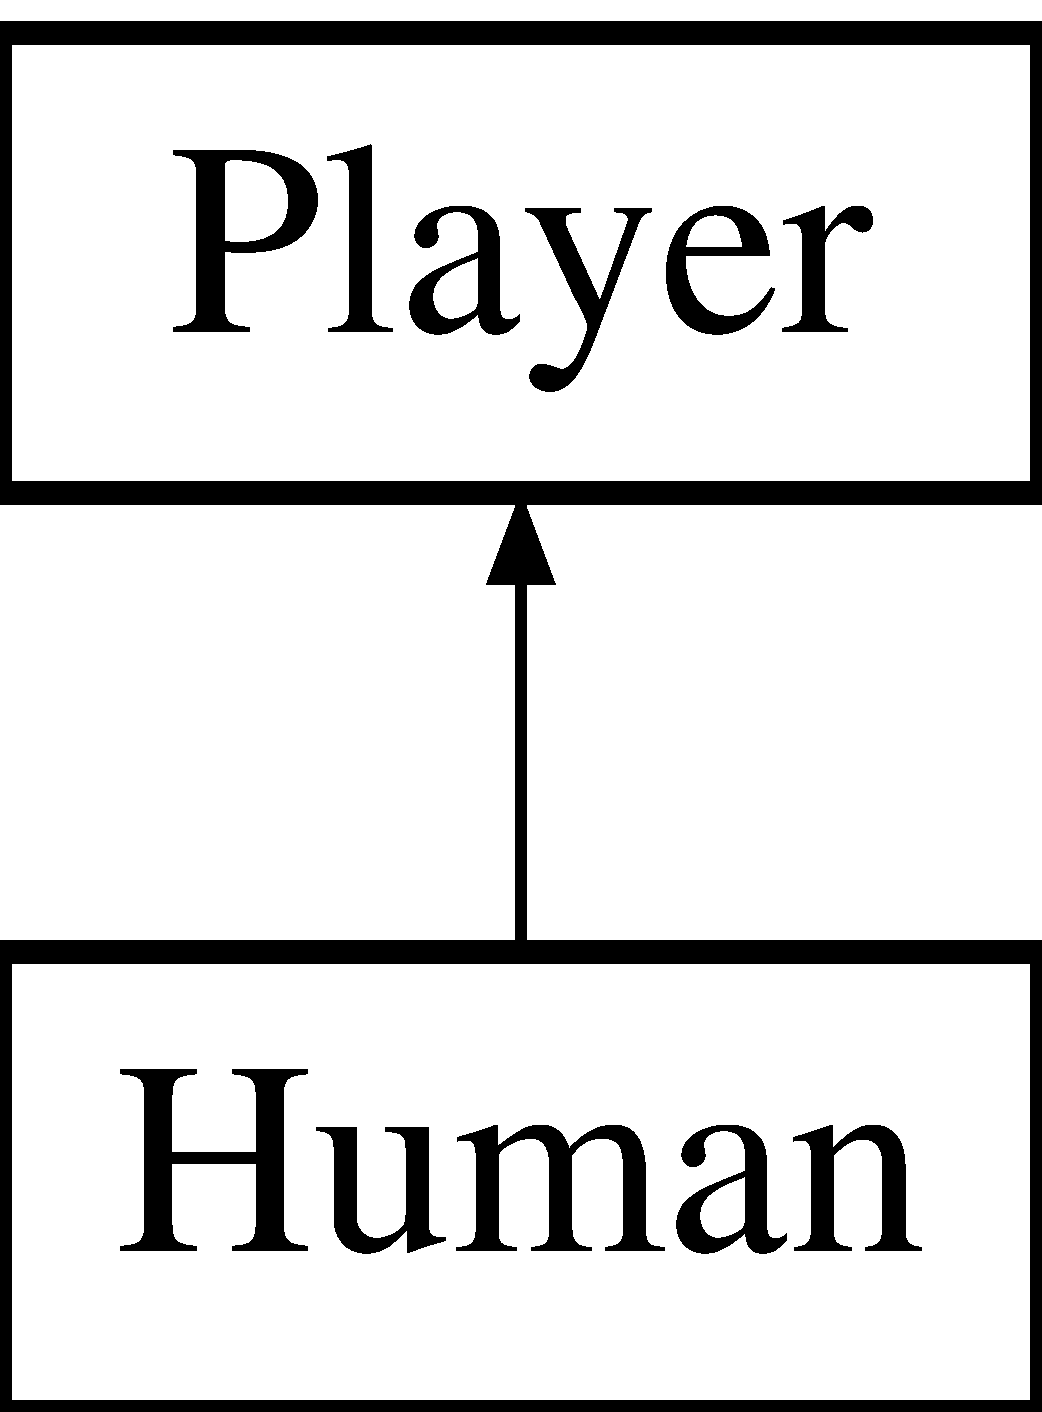
\includegraphics[height=2.000000cm]{classHuman}
\end{center}
\end{figure}
\subsection*{Public Member Functions}
\begin{DoxyCompactItemize}
\item 
\hyperlink{classHuman_abfd57b90d90f9222384c76b44346ba7b}{Human} (const string \&\hyperlink{classPlayer_acf0355128a99ee20ad9931b760fb2de1}{name})
\begin{DoxyCompactList}\small\item\em The unique constructor of \hyperlink{classHuman}{Human}. \end{DoxyCompactList}\item 
shared\-\_\-ptr$<$ \hyperlink{classCard}{Card} $>$ \hyperlink{classHuman_a3258d3ce0eec7a5e393c639506ef28e5}{play\-Card} (shared\-\_\-ptr$<$ \hyperlink{classCard}{Card} $>$ reference\-Card, shared\-\_\-ptr$<$ \hyperlink{classCard}{Card} $>$ high\-Trump)
\begin{DoxyCompactList}\small\item\em To play a card, knowing the ask suit and the highest trump of the trick, if any. \end{DoxyCompactList}\item 
\hypertarget{classHuman_aae5efb6945fdbcda9c9a4d9e72d4a60e}{void \hyperlink{classHuman_aae5efb6945fdbcda9c9a4d9e72d4a60e}{new\-Game} ()}\label{classHuman_aae5efb6945fdbcda9c9a4d9e72d4a60e}

\begin{DoxyCompactList}\small\item\em To get prepared for a new game. \end{DoxyCompactList}\item 
Biddings \hyperlink{classHuman_a424bc9179b7036f22a694329b5f6fedf}{bid} (const Biddings best\-Bid, const bool chelem\-Announced) const 
\begin{DoxyCompactList}\small\item\em To let the \hyperlink{classHuman}{Human} player bids. \end{DoxyCompactList}\item 
shared\-\_\-ptr$<$ \hyperlink{classCard}{Card} $>$ \hyperlink{classHuman_a7b465bef30158c2b5552f54651e48318}{choose\-King} (const \hyperlink{classDeck}{Deck} \&deck) const 
\begin{DoxyCompactList}\small\item\em To make a choice for partnership in a 5-\/player game. \end{DoxyCompactList}\item 
set$<$ shared\-\_\-ptr$<$ \hyperlink{classCard}{Card} $>$ $>$ \hyperlink{classHuman_a02cdef89dde0adcb554f081e81f97896}{make\-Ecart} (const int dog\-Size)
\begin{DoxyCompactList}\small\item\em To let the \hyperlink{classHuman}{Human} player makes his/her ecart. \end{DoxyCompactList}\end{DoxyCompactItemize}
\subsection*{Additional Inherited Members}


\subsection{Detailed Description}
\hyperlink{classHuman}{Human} is the class implementing \hyperlink{classHuman}{Human} player actions, like playing a card. 

\subsection{Constructor \& Destructor Documentation}
\hypertarget{classHuman_abfd57b90d90f9222384c76b44346ba7b}{\index{Human@{Human}!Human@{Human}}
\index{Human@{Human}!Human@{Human}}
\subsubsection[{Human}]{\setlength{\rightskip}{0pt plus 5cm}Human\-::\-Human (
\begin{DoxyParamCaption}
\item[{const string \&}]{name}
\end{DoxyParamCaption}
)}}\label{classHuman_abfd57b90d90f9222384c76b44346ba7b}


The unique constructor of \hyperlink{classHuman}{Human}. 


\begin{DoxyParams}{Parameters}
{\em name} & The name of the \hyperlink{classHuman}{Human} player. \\
\hline
\end{DoxyParams}


\subsection{Member Function Documentation}
\hypertarget{classHuman_a424bc9179b7036f22a694329b5f6fedf}{\index{Human@{Human}!bid@{bid}}
\index{bid@{bid}!Human@{Human}}
\subsubsection[{bid}]{\setlength{\rightskip}{0pt plus 5cm}Biddings Human\-::bid (
\begin{DoxyParamCaption}
\item[{const Biddings}]{best\-Bid, }
\item[{const bool}]{chelem\-Announced}
\end{DoxyParamCaption}
) const\hspace{0.3cm}{\ttfamily [virtual]}}}\label{classHuman_a424bc9179b7036f22a694329b5f6fedf}


To let the \hyperlink{classHuman}{Human} player bids. 


\begin{DoxyParams}{Parameters}
{\em best\-Bid} & The best bid proposed so far. \\
\hline
{\em chelem\-Announced} & True iff a chelem has been announced. \\
\hline
\end{DoxyParams}
\begin{DoxyReturn}{Returns}
The \hyperlink{classHuman}{Human} player's bid. 
\end{DoxyReturn}


Implements \hyperlink{classPlayer_a4bb658ca7b46f32a42578b884ad7fe82}{Player}.

\hypertarget{classHuman_a7b465bef30158c2b5552f54651e48318}{\index{Human@{Human}!choose\-King@{choose\-King}}
\index{choose\-King@{choose\-King}!Human@{Human}}
\subsubsection[{choose\-King}]{\setlength{\rightskip}{0pt plus 5cm}shared\-\_\-ptr$<$ {\bf Card} $>$ Human\-::choose\-King (
\begin{DoxyParamCaption}
\item[{const {\bf Deck} \&}]{deck}
\end{DoxyParamCaption}
) const\hspace{0.3cm}{\ttfamily [virtual]}}}\label{classHuman_a7b465bef30158c2b5552f54651e48318}


To make a choice for partnership in a 5-\/player game. 


\begin{DoxyParams}{Parameters}
{\em deck} & The current deck used for the game \\
\hline
\end{DoxyParams}
\begin{DoxyReturn}{Returns}
The chosen king (or card). 
\end{DoxyReturn}


Implements \hyperlink{classPlayer_ac85ce39f638b28f13588e8957dc952ff}{Player}.

\hypertarget{classHuman_a02cdef89dde0adcb554f081e81f97896}{\index{Human@{Human}!make\-Ecart@{make\-Ecart}}
\index{make\-Ecart@{make\-Ecart}!Human@{Human}}
\subsubsection[{make\-Ecart}]{\setlength{\rightskip}{0pt plus 5cm}set$<$ shared\-\_\-ptr$<$ {\bf Card} $>$ $>$ Human\-::make\-Ecart (
\begin{DoxyParamCaption}
\item[{const int}]{dog\-Size}
\end{DoxyParamCaption}
)\hspace{0.3cm}{\ttfamily [virtual]}}}\label{classHuman_a02cdef89dde0adcb554f081e81f97896}


To let the \hyperlink{classHuman}{Human} player makes his/her ecart. 


\begin{DoxyParams}{Parameters}
{\em dog\-Size} & The number of cards to put into the ecart. \\
\hline
\end{DoxyParams}


Implements \hyperlink{classPlayer_a34c9e9f402c6a68d6e16caebdb93a33f}{Player}.

\hypertarget{classHuman_a3258d3ce0eec7a5e393c639506ef28e5}{\index{Human@{Human}!play\-Card@{play\-Card}}
\index{play\-Card@{play\-Card}!Human@{Human}}
\subsubsection[{play\-Card}]{\setlength{\rightskip}{0pt plus 5cm}shared\-\_\-ptr$<$ {\bf Card} $>$ Human\-::play\-Card (
\begin{DoxyParamCaption}
\item[{shared\-\_\-ptr$<$ {\bf Card} $>$}]{reference\-Card, }
\item[{shared\-\_\-ptr$<$ {\bf Card} $>$}]{high\-Trump}
\end{DoxyParamCaption}
)\hspace{0.3cm}{\ttfamily [virtual]}}}\label{classHuman_a3258d3ce0eec7a5e393c639506ef28e5}


To play a card, knowing the ask suit and the highest trump of the trick, if any. 


\begin{DoxyParams}{Parameters}
{\em reference\-Card} & The card fixing the ask suit for the trick. \\
\hline
{\em high\-Trump} & The highest trump played so far for the trick, if any. \\
\hline
\end{DoxyParams}
\begin{DoxyReturn}{Returns}
The card the player plays. 
\end{DoxyReturn}


Implements \hyperlink{classPlayer_aeba090a124bfd9a3666d2d793439cae0}{Player}.



The documentation for this class was generated from the following files\-:\begin{DoxyCompactItemize}
\item 
src/Human.\-hpp\item 
src/Human.\-cpp\end{DoxyCompactItemize}

\hypertarget{classPlayer}{\section{Player Class Reference}
\label{classPlayer}\index{Player@{Player}}
}


\hyperlink{classPlayer}{Player} is an abstract class presenting a common interface for \hyperlink{classAI}{A\-I} and \hyperlink{classHuman}{Human} players.  




{\ttfamily \#include $<$Player.\-hpp$>$}

Inheritance diagram for Player\-:\begin{figure}[H]
\begin{center}
\leavevmode
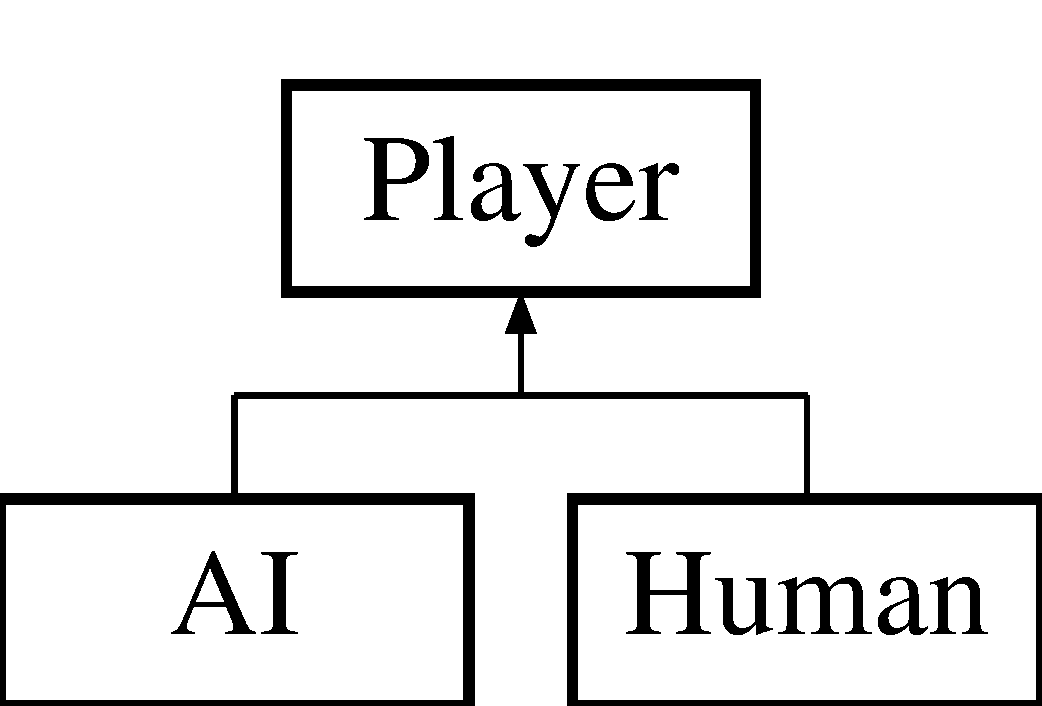
\includegraphics[height=2.000000cm]{classPlayer}
\end{center}
\end{figure}
\subsection*{Classes}
\begin{DoxyCompactItemize}
\item 
struct \hyperlink{structPlayer_1_1cardOrder}{card\-Order}
\begin{DoxyCompactList}\small\item\em A structure to automatically fix an insert order into cards' sets. \end{DoxyCompactList}\end{DoxyCompactItemize}
\subsection*{Public Member Functions}
\begin{DoxyCompactItemize}
\item 
\hyperlink{classPlayer_a5a2790fccf10c30106370d910c96d317}{Player} (const string \&\hyperlink{classPlayer_acf0355128a99ee20ad9931b760fb2de1}{name})
\begin{DoxyCompactList}\small\item\em The unique constructor of \hyperlink{classPlayer}{Player}. \end{DoxyCompactList}\item 
virtual shared\-\_\-ptr$<$ \hyperlink{classCard}{Card} $>$ \hyperlink{classPlayer_aeba090a124bfd9a3666d2d793439cae0}{play\-Card} (shared\-\_\-ptr$<$ \hyperlink{classCard}{Card} $>$ reference\-Card, shared\-\_\-ptr$<$ \hyperlink{classCard}{Card} $>$ high\-Trump)=0
\begin{DoxyCompactList}\small\item\em play\-Card is a pure virtual function returning the card the player chooses to play. \end{DoxyCompactList}\item 
\hypertarget{classPlayer_a76a707ceb6f24b0a2a801434ee5a60ad}{virtual void \hyperlink{classPlayer_a76a707ceb6f24b0a2a801434ee5a60ad}{new\-Game} ()=0}\label{classPlayer_a76a707ceb6f24b0a2a801434ee5a60ad}

\begin{DoxyCompactList}\small\item\em Pure virtual function to prepare the player for a new game. \end{DoxyCompactList}\item 
virtual Biddings \hyperlink{classPlayer_a4bb658ca7b46f32a42578b884ad7fe82}{bid} (const Biddings best\-Bid, const bool chelem\-Announced) const =0
\begin{DoxyCompactList}\small\item\em Pure virtual function to make a choice for biddings. \end{DoxyCompactList}\item 
virtual shared\-\_\-ptr$<$ \hyperlink{classCard}{Card} $>$ \hyperlink{classPlayer_ac85ce39f638b28f13588e8957dc952ff}{choose\-King} (const \hyperlink{classDeck}{Deck} \&deck) const =0
\begin{DoxyCompactList}\small\item\em Pure virtual function to make a choice for partnership in a 5-\/player game. \end{DoxyCompactList}\item 
virtual set$<$ shared\-\_\-ptr$<$ \hyperlink{classCard}{Card} $>$ $>$ \hyperlink{classPlayer_a34c9e9f402c6a68d6e16caebdb93a33f}{make\-Ecart} (const int dog\-Size)=0
\begin{DoxyCompactList}\small\item\em Pure virtual function to make the ecart when the player is the best bidder. \end{DoxyCompactList}\item 
\hypertarget{classPlayer_a5573dd91ddb6fa8874d5a7f7a186f186}{set$<$ Announcements $>$ \hyperlink{classPlayer_a5573dd91ddb6fa8874d5a7f7a186f186}{get\-Announced} () const }\label{classPlayer_a5573dd91ddb6fa8874d5a7f7a186f186}

\begin{DoxyCompactList}\small\item\em Inline assessor to the set of announcements. \end{DoxyCompactList}\item 
\hypertarget{classPlayer_a4dc51cf2a773556eb26f3d47c4274b0a}{int \hyperlink{classPlayer_a4dc51cf2a773556eb26f3d47c4274b0a}{get\-Number\-Oudlers} () const }\label{classPlayer_a4dc51cf2a773556eb26f3d47c4274b0a}

\begin{DoxyCompactList}\small\item\em Inline assessor to the number of oudlers the player has with his/her initial hand. \end{DoxyCompactList}\item 
\hypertarget{classPlayer_aab2cfa2ce2e7a3903ff99ac5c7ef8db6}{vector$<$ shared\-\_\-ptr$<$ \hyperlink{classCard}{Card} $>$ $>$ \hyperlink{classPlayer_aab2cfa2ce2e7a3903ff99ac5c7ef8db6}{get\-Initial\-Cards} () const }\label{classPlayer_aab2cfa2ce2e7a3903ff99ac5c7ef8db6}

\begin{DoxyCompactList}\small\item\em Inline assessor to the player's initial cards. \end{DoxyCompactList}\item 
vector$<$ shared\-\_\-ptr$<$ \hyperlink{classCard}{Card} $>$ $>$ \hyperlink{classPlayer_ab89873d894a8e4e7e67a16feba4bf116}{valid\-Cards} (shared\-\_\-ptr$<$ \hyperlink{classCard}{Card} $>$ ref\-Card, shared\-\_\-ptr$<$ \hyperlink{classCard}{Card} $>$ greater\-Trump)
\begin{DoxyCompactList}\small\item\em Returns the vector of cards the player can currently play, regarding the asked suit and the greater trump of the trick. \end{DoxyCompactList}\item 
void \hyperlink{classPlayer_a7c7b8325247c91ef255ca493de9f35eb}{add\-Card} (shared\-\_\-ptr$<$ \hyperlink{classCard}{Card} $>$ card)
\begin{DoxyCompactList}\small\item\em Add a card among player's initial cards. \end{DoxyCompactList}\item 
\hypertarget{classPlayer_a5216f487067dd79371af457f4b8f1769}{void \hyperlink{classPlayer_a5216f487067dd79371af457f4b8f1769}{show\-Cards} () const }\label{classPlayer_a5216f487067dd79371af457f4b8f1769}

\begin{DoxyCompactList}\small\item\em To print all player's cards in his/her current hand. \end{DoxyCompactList}\end{DoxyCompactItemize}
\subsection*{Public Attributes}
\begin{DoxyCompactItemize}
\item 
\hypertarget{classPlayer_acf0355128a99ee20ad9931b760fb2de1}{string \hyperlink{classPlayer_acf0355128a99ee20ad9931b760fb2de1}{name}}\label{classPlayer_acf0355128a99ee20ad9931b760fb2de1}

\begin{DoxyCompactList}\small\item\em The player's name. \end{DoxyCompactList}\item 
\hypertarget{classPlayer_a55f7b5b674245c2e09f3c191a54d3542}{double \hyperlink{classPlayer_a55f7b5b674245c2e09f3c191a54d3542}{score}}\label{classPlayer_a55f7b5b674245c2e09f3c191a54d3542}

\begin{DoxyCompactList}\small\item\em The player's score. \end{DoxyCompactList}\end{DoxyCompactItemize}
\subsection*{Protected Member Functions}
\begin{DoxyCompactItemize}
\item 
void \hyperlink{classPlayer_a82c40ddca5214bbc9cc204ae9b789ca7}{del\-Card} (shared\-\_\-ptr$<$ \hyperlink{classCard}{Card} $>$ card)
\begin{DoxyCompactList}\small\item\em To delete a card from the player's current hand. \end{DoxyCompactList}\item 
vector$<$ shared\-\_\-ptr$<$ \hyperlink{classCard}{Card} $>$ $>$ \hyperlink{classPlayer_a2880662cb5f5cc2e778242c7a1477b30}{callable\-Cards} (const \hyperlink{classDeck}{Deck} \&deck) const 
\begin{DoxyCompactList}\small\item\em To compute the vector of cards we can call during a 5-\/player game. \end{DoxyCompactList}\end{DoxyCompactItemize}
\subsection*{Protected Attributes}
\begin{DoxyCompactItemize}
\item 
\hypertarget{classPlayer_afab8e372cfef87440bc42168d5fa0f6a}{set$<$ shared\-\_\-ptr$<$ \hyperlink{classCard}{Card} $>$\\*
, \hyperlink{structPlayer_1_1cardOrder}{card\-Order} $>$ \hyperlink{classPlayer_afab8e372cfef87440bc42168d5fa0f6a}{hearts}}\label{classPlayer_afab8e372cfef87440bc42168d5fa0f6a}

\begin{DoxyCompactList}\small\item\em The set of Hearts owned by the player. \end{DoxyCompactList}\item 
\hypertarget{classPlayer_a89177ee8076c1a3411a74b2b1d68156c}{set$<$ shared\-\_\-ptr$<$ \hyperlink{classCard}{Card} $>$\\*
, \hyperlink{structPlayer_1_1cardOrder}{card\-Order} $>$ \hyperlink{classPlayer_a89177ee8076c1a3411a74b2b1d68156c}{spades}}\label{classPlayer_a89177ee8076c1a3411a74b2b1d68156c}

\begin{DoxyCompactList}\small\item\em The set of Spades owned by the player. \end{DoxyCompactList}\item 
\hypertarget{classPlayer_a3ad0f1545e0653635eac5ced5c31dc0b}{set$<$ shared\-\_\-ptr$<$ \hyperlink{classCard}{Card} $>$\\*
, \hyperlink{structPlayer_1_1cardOrder}{card\-Order} $>$ \hyperlink{classPlayer_a3ad0f1545e0653635eac5ced5c31dc0b}{diamonds}}\label{classPlayer_a3ad0f1545e0653635eac5ced5c31dc0b}

\begin{DoxyCompactList}\small\item\em The set of Diamonds owned by the player. \end{DoxyCompactList}\item 
\hypertarget{classPlayer_ad3f3acdaf6ee318ba528e82e1c188820}{set$<$ shared\-\_\-ptr$<$ \hyperlink{classCard}{Card} $>$\\*
, \hyperlink{structPlayer_1_1cardOrder}{card\-Order} $>$ \hyperlink{classPlayer_ad3f3acdaf6ee318ba528e82e1c188820}{clubs}}\label{classPlayer_ad3f3acdaf6ee318ba528e82e1c188820}

\begin{DoxyCompactList}\small\item\em The set of Clubs owned by the player. \end{DoxyCompactList}\item 
\hypertarget{classPlayer_a66b3455fc8c6685a78eb193a015a07a0}{set$<$ shared\-\_\-ptr$<$ \hyperlink{classCard}{Card} $>$\\*
, \hyperlink{structPlayer_1_1cardOrder}{card\-Order} $>$ \hyperlink{classPlayer_a66b3455fc8c6685a78eb193a015a07a0}{trumps}}\label{classPlayer_a66b3455fc8c6685a78eb193a015a07a0}

\begin{DoxyCompactList}\small\item\em The set of trumps owned by the player. \end{DoxyCompactList}\item 
\hypertarget{classPlayer_a9dfead246bd18b99398c89777290a162}{shared\-\_\-ptr$<$ \hyperlink{classCard}{Card} $>$ \hyperlink{classPlayer_a9dfead246bd18b99398c89777290a162}{fool}}\label{classPlayer_a9dfead246bd18b99398c89777290a162}

\begin{DoxyCompactList}\small\item\em The pointer toward the Fool, if owned by the player. \end{DoxyCompactList}\item 
\hypertarget{classPlayer_aac0d154d58a07310ee23c3c763f2cfa9}{vector$<$ shared\-\_\-ptr$<$ \hyperlink{classCard}{Card} $>$ $>$ \hyperlink{classPlayer_aac0d154d58a07310ee23c3c763f2cfa9}{initial\-Cards}}\label{classPlayer_aac0d154d58a07310ee23c3c763f2cfa9}

\begin{DoxyCompactList}\small\item\em The vector of player's initial cards, from his/her starting hand. \end{DoxyCompactList}\item 
\hypertarget{classPlayer_a9f218c1ff377eaeb7a336156410f7386}{int \hyperlink{classPlayer_a9f218c1ff377eaeb7a336156410f7386}{number\-Oudlers}}\label{classPlayer_a9f218c1ff377eaeb7a336156410f7386}

\begin{DoxyCompactList}\small\item\em The number of oudlers the player has among his/her initial cards. \end{DoxyCompactList}\item 
\hypertarget{classPlayer_af625acf7f8ad267630c7e3bd50d2683b}{double \hyperlink{classPlayer_af625acf7f8ad267630c7e3bd50d2683b}{initial\-Points}}\label{classPlayer_af625acf7f8ad267630c7e3bd50d2683b}

\begin{DoxyCompactList}\small\item\em The number of points the player has with his/her initial cards. \end{DoxyCompactList}\item 
\hypertarget{classPlayer_a90efe0cf8930297c7d30805d19763b65}{set$<$ Announcements $>$ \hyperlink{classPlayer_a90efe0cf8930297c7d30805d19763b65}{announced}}\label{classPlayer_a90efe0cf8930297c7d30805d19763b65}

\begin{DoxyCompactList}\small\item\em The set of announcements (for what?). \end{DoxyCompactList}\end{DoxyCompactItemize}


\subsection{Detailed Description}
\hyperlink{classPlayer}{Player} is an abstract class presenting a common interface for \hyperlink{classAI}{A\-I} and \hyperlink{classHuman}{Human} players. 

\subsection{Constructor \& Destructor Documentation}
\hypertarget{classPlayer_a5a2790fccf10c30106370d910c96d317}{\index{Player@{Player}!Player@{Player}}
\index{Player@{Player}!Player@{Player}}
\subsubsection[{Player}]{\setlength{\rightskip}{0pt plus 5cm}Player\-::\-Player (
\begin{DoxyParamCaption}
\item[{const string \&}]{name}
\end{DoxyParamCaption}
)}}\label{classPlayer_a5a2790fccf10c30106370d910c96d317}


The unique constructor of \hyperlink{classPlayer}{Player}. 


\begin{DoxyParams}{Parameters}
{\em name} & The player name. \\
\hline
\end{DoxyParams}


\subsection{Member Function Documentation}
\hypertarget{classPlayer_a7c7b8325247c91ef255ca493de9f35eb}{\index{Player@{Player}!add\-Card@{add\-Card}}
\index{add\-Card@{add\-Card}!Player@{Player}}
\subsubsection[{add\-Card}]{\setlength{\rightskip}{0pt plus 5cm}void Player\-::add\-Card (
\begin{DoxyParamCaption}
\item[{shared\-\_\-ptr$<$ {\bf Card} $>$}]{card}
\end{DoxyParamCaption}
)}}\label{classPlayer_a7c7b8325247c91ef255ca493de9f35eb}


Add a card among player's initial cards. 


\begin{DoxyParams}{Parameters}
{\em card} & The card to add. \\
\hline
\end{DoxyParams}
\hypertarget{classPlayer_a4bb658ca7b46f32a42578b884ad7fe82}{\index{Player@{Player}!bid@{bid}}
\index{bid@{bid}!Player@{Player}}
\subsubsection[{bid}]{\setlength{\rightskip}{0pt plus 5cm}virtual Biddings Player\-::bid (
\begin{DoxyParamCaption}
\item[{const Biddings}]{best\-Bid, }
\item[{const bool}]{chelem\-Announced}
\end{DoxyParamCaption}
) const\hspace{0.3cm}{\ttfamily [pure virtual]}}}\label{classPlayer_a4bb658ca7b46f32a42578b884ad7fe82}


Pure virtual function to make a choice for biddings. 


\begin{DoxyParams}{Parameters}
{\em best\-Bid} & The best bid proposed so far. \\
\hline
{\em chelem\-Announced} & A Boolean to know if someone has declared a chelem. \\
\hline
\end{DoxyParams}
\begin{DoxyReturn}{Returns}
The chosen bid (Biddings\-::none if one passes). 
\end{DoxyReturn}


Implemented in \hyperlink{classAI_a9e2fd7ff440ada8339135c23b73e1a96}{A\-I}, and \hyperlink{classHuman_a424bc9179b7036f22a694329b5f6fedf}{Human}.

\hypertarget{classPlayer_a2880662cb5f5cc2e778242c7a1477b30}{\index{Player@{Player}!callable\-Cards@{callable\-Cards}}
\index{callable\-Cards@{callable\-Cards}!Player@{Player}}
\subsubsection[{callable\-Cards}]{\setlength{\rightskip}{0pt plus 5cm}vector$<$ shared\-\_\-ptr$<$ {\bf Card} $>$ $>$ Player\-::callable\-Cards (
\begin{DoxyParamCaption}
\item[{const {\bf Deck} \&}]{deck}
\end{DoxyParamCaption}
) const\hspace{0.3cm}{\ttfamily [protected]}}}\label{classPlayer_a2880662cb5f5cc2e778242c7a1477b30}


To compute the vector of cards we can call during a 5-\/player game. 


\begin{DoxyParams}{Parameters}
{\em deck} & The deck used form the game. \\
\hline
\end{DoxyParams}
\begin{DoxyReturn}{Returns}
the vector of cards the taker can call (usually, the four kings). 
\end{DoxyReturn}
\hypertarget{classPlayer_ac85ce39f638b28f13588e8957dc952ff}{\index{Player@{Player}!choose\-King@{choose\-King}}
\index{choose\-King@{choose\-King}!Player@{Player}}
\subsubsection[{choose\-King}]{\setlength{\rightskip}{0pt plus 5cm}virtual shared\-\_\-ptr$<${\bf Card}$>$ Player\-::choose\-King (
\begin{DoxyParamCaption}
\item[{const {\bf Deck} \&}]{deck}
\end{DoxyParamCaption}
) const\hspace{0.3cm}{\ttfamily [pure virtual]}}}\label{classPlayer_ac85ce39f638b28f13588e8957dc952ff}


Pure virtual function to make a choice for partnership in a 5-\/player game. 


\begin{DoxyParams}{Parameters}
{\em deck} & The current deck used for the game \\
\hline
\end{DoxyParams}
\begin{DoxyReturn}{Returns}
The chosen king (or card). 
\end{DoxyReturn}


Implemented in \hyperlink{classAI_a6d7eafe5efa20fd78ec91048ad7c1ae2}{A\-I}, and \hyperlink{classHuman_a7b465bef30158c2b5552f54651e48318}{Human}.

\hypertarget{classPlayer_a82c40ddca5214bbc9cc204ae9b789ca7}{\index{Player@{Player}!del\-Card@{del\-Card}}
\index{del\-Card@{del\-Card}!Player@{Player}}
\subsubsection[{del\-Card}]{\setlength{\rightskip}{0pt plus 5cm}void Player\-::del\-Card (
\begin{DoxyParamCaption}
\item[{shared\-\_\-ptr$<$ {\bf Card} $>$}]{card}
\end{DoxyParamCaption}
)\hspace{0.3cm}{\ttfamily [protected]}}}\label{classPlayer_a82c40ddca5214bbc9cc204ae9b789ca7}


To delete a card from the player's current hand. 


\begin{DoxyParams}{Parameters}
{\em card} & The card to delete from the player's hand. \\
\hline
\end{DoxyParams}
\hypertarget{classPlayer_a34c9e9f402c6a68d6e16caebdb93a33f}{\index{Player@{Player}!make\-Ecart@{make\-Ecart}}
\index{make\-Ecart@{make\-Ecart}!Player@{Player}}
\subsubsection[{make\-Ecart}]{\setlength{\rightskip}{0pt plus 5cm}virtual set$<$ shared\-\_\-ptr$<${\bf Card}$>$ $>$ Player\-::make\-Ecart (
\begin{DoxyParamCaption}
\item[{const int}]{dog\-Size}
\end{DoxyParamCaption}
)\hspace{0.3cm}{\ttfamily [pure virtual]}}}\label{classPlayer_a34c9e9f402c6a68d6e16caebdb93a33f}


Pure virtual function to make the ecart when the player is the best bidder. 


\begin{DoxyParams}{Parameters}
{\em dog\-Size} & The number of card one must include into the ecart. \\
\hline
\end{DoxyParams}
\begin{DoxyReturn}{Returns}
A set of \hyperlink{classCard}{Card} pointers for the cards one places into the ecart. 
\end{DoxyReturn}


Implemented in \hyperlink{classAI_ad12a3efd1da4acc6e1855bd7262779e3}{A\-I}, and \hyperlink{classHuman_a02cdef89dde0adcb554f081e81f97896}{Human}.

\hypertarget{classPlayer_aeba090a124bfd9a3666d2d793439cae0}{\index{Player@{Player}!play\-Card@{play\-Card}}
\index{play\-Card@{play\-Card}!Player@{Player}}
\subsubsection[{play\-Card}]{\setlength{\rightskip}{0pt plus 5cm}virtual shared\-\_\-ptr$<${\bf Card}$>$ Player\-::play\-Card (
\begin{DoxyParamCaption}
\item[{shared\-\_\-ptr$<$ {\bf Card} $>$}]{reference\-Card, }
\item[{shared\-\_\-ptr$<$ {\bf Card} $>$}]{high\-Trump}
\end{DoxyParamCaption}
)\hspace{0.3cm}{\ttfamily [pure virtual]}}}\label{classPlayer_aeba090a124bfd9a3666d2d793439cae0}


play\-Card is a pure virtual function returning the card the player chooses to play. 


\begin{DoxyParams}{Parameters}
{\em reference\-Card} & The card fixing the ask suit for the trick. \\
\hline
{\em high\-Trump} & The highest trump played so far for the trick, if any. \\
\hline
\end{DoxyParams}
\begin{DoxyReturn}{Returns}
The chosen card to play. 
\end{DoxyReturn}


Implemented in \hyperlink{classAI_a3f5b2888e03634db701c66f82a4f03a8}{A\-I}, and \hyperlink{classHuman_a3258d3ce0eec7a5e393c639506ef28e5}{Human}.

\hypertarget{classPlayer_ab89873d894a8e4e7e67a16feba4bf116}{\index{Player@{Player}!valid\-Cards@{valid\-Cards}}
\index{valid\-Cards@{valid\-Cards}!Player@{Player}}
\subsubsection[{valid\-Cards}]{\setlength{\rightskip}{0pt plus 5cm}vector$<$ shared\-\_\-ptr$<$ {\bf Card} $>$ $>$ Player\-::valid\-Cards (
\begin{DoxyParamCaption}
\item[{shared\-\_\-ptr$<$ {\bf Card} $>$}]{ref\-Card, }
\item[{shared\-\_\-ptr$<$ {\bf Card} $>$}]{greater\-Trump}
\end{DoxyParamCaption}
)}}\label{classPlayer_ab89873d894a8e4e7e67a16feba4bf116}


Returns the vector of cards the player can currently play, regarding the asked suit and the greater trump of the trick. 


\begin{DoxyParams}{Parameters}
{\em ref\-Card} & A pointer of the card fixing the asked suit of the trick. \\
\hline
{\em greater\-Trump} & A pointer on the greater trump of the trick, if any. \\
\hline
\end{DoxyParams}
\begin{DoxyReturn}{Returns}
The vector of all cards the player can play in his/her situation. 
\end{DoxyReturn}


The documentation for this class was generated from the following files\-:\begin{DoxyCompactItemize}
\item 
src/Player.\-hpp\item 
src/Player.\-cpp\end{DoxyCompactItemize}

\hypertarget{classStratDiff}{\section{\-Strat\-Diff \-Class \-Reference}
\label{classStratDiff}\index{\-Strat\-Diff@{\-Strat\-Diff}}
}


\hyperlink{classStratDiff}{\-Strat\-Diff} is the abstract class handling the \-Strategy pattern for applying different \hyperlink{classAI}{\-A\-I} difficulties.  




{\ttfamily \#include $<$\-Strat\-Diff.\-hpp$>$}

\-Inheritance diagram for \-Strat\-Diff\-:\begin{figure}[H]
\begin{center}
\leavevmode
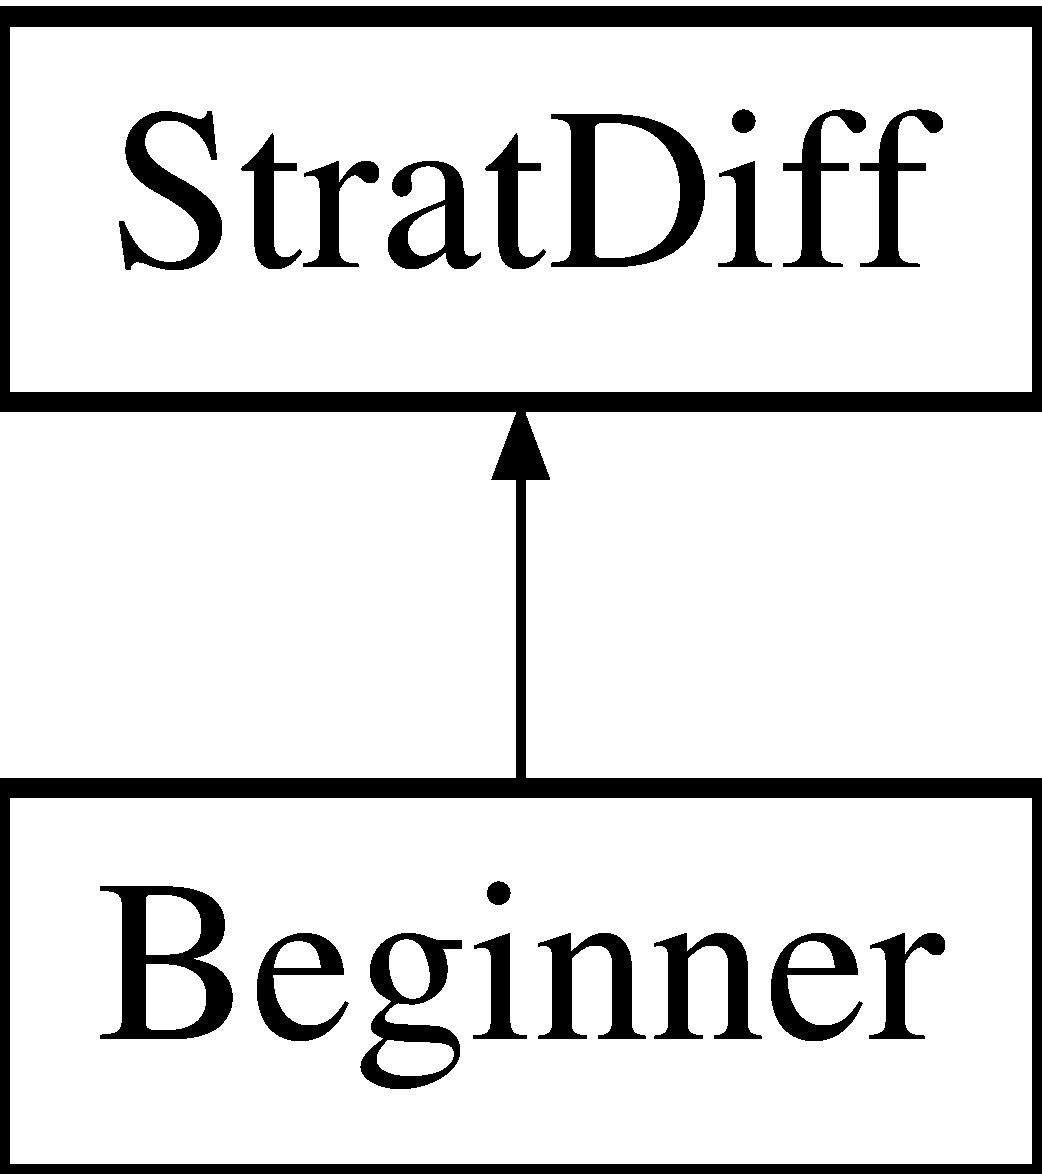
\includegraphics[height=2.000000cm]{classStratDiff}
\end{center}
\end{figure}
\subsection*{\-Public \-Member \-Functions}
\begin{DoxyCompactItemize}
\item 
virtual shared\-\_\-ptr$<$ \hyperlink{classCard}{\-Card} $>$ \hyperlink{classStratDiff_a7882bac82aa02692bf5e6b33e9c4ae6c}{play\-Card} (vector$<$ shared\-\_\-ptr$<$ \hyperlink{classCard}{\-Card} $>$ $>$ cards\-Can\-Play)=0
\begin{DoxyCompactList}\small\item\em play\-Card is a pure virtual function returning the card the player chooses to play. \end{DoxyCompactList}\item 
virtual \-Biddings \hyperlink{classStratDiff_a84fc8f51747065234c9356895057008b}{bid} (\-Biddings best\-Bid, int number\-Oudlers, bool chelem\-Announced)=0
\begin{DoxyCompactList}\small\item\em \-Called to decide if we propose a bid or not, and if any, what bid. \end{DoxyCompactList}\item 
virtual set$<$ shared\-\_\-ptr$<$ \hyperlink{classCard}{\-Card} $>$ $>$ \hyperlink{classStratDiff_aec61f7e84d1376d41f13d044b3672226}{make\-Ecart} (int dog\-Size, vector$<$ shared\-\_\-ptr$<$ \hyperlink{classCard}{\-Card} $>$ $>$ all\-Cards)=0
\begin{DoxyCompactList}\small\item\em \-To make the ecart once we take the dog. \end{DoxyCompactList}\end{DoxyCompactItemize}


\subsection{\-Detailed \-Description}
\hyperlink{classStratDiff}{\-Strat\-Diff} is the abstract class handling the \-Strategy pattern for applying different \hyperlink{classAI}{\-A\-I} difficulties. 

\subsection{\-Member \-Function \-Documentation}
\hypertarget{classStratDiff_a84fc8f51747065234c9356895057008b}{\index{\-Strat\-Diff@{\-Strat\-Diff}!bid@{bid}}
\index{bid@{bid}!StratDiff@{\-Strat\-Diff}}
\subsubsection[{bid}]{\setlength{\rightskip}{0pt plus 5cm}virtual \-Biddings {\bf \-Strat\-Diff\-::bid} (
\begin{DoxyParamCaption}
\item[{\-Biddings}]{best\-Bid, }
\item[{int}]{number\-Oudlers, }
\item[{bool}]{chelem\-Announced}
\end{DoxyParamCaption}
)\hspace{0.3cm}{\ttfamily  \mbox{[}pure virtual\mbox{]}}}}\label{classStratDiff_a84fc8f51747065234c9356895057008b}


\-Called to decide if we propose a bid or not, and if any, what bid. 


\begin{DoxyParams}{\-Parameters}
{\em best\-Bid} & \-The best bid proposed so far. \\
\hline
{\em number\-Oudlers} & \-The number of oudlers we have in our hand. \\
\hline
{\em chelem\-Announced} & \-A \-Boolean to know if someone has declared a chelem. \\
\hline
\end{DoxyParams}
\begin{DoxyReturn}{\-Returns}
\-Our bid (\-Biddings\-::none if we pass). 
\end{DoxyReturn}


\-Implemented in \hyperlink{classBeginner_a742825d7c3629507b7486f7bb9ae5544}{\-Beginner}.

\hypertarget{classStratDiff_aec61f7e84d1376d41f13d044b3672226}{\index{\-Strat\-Diff@{\-Strat\-Diff}!make\-Ecart@{make\-Ecart}}
\index{make\-Ecart@{make\-Ecart}!StratDiff@{\-Strat\-Diff}}
\subsubsection[{make\-Ecart}]{\setlength{\rightskip}{0pt plus 5cm}virtual set$<$ shared\-\_\-ptr$<${\bf \-Card}$>$ $>$ {\bf \-Strat\-Diff\-::make\-Ecart} (
\begin{DoxyParamCaption}
\item[{int}]{dog\-Size, }
\item[{vector$<$ shared\-\_\-ptr$<$ {\bf \-Card} $>$ $>$}]{all\-Cards}
\end{DoxyParamCaption}
)\hspace{0.3cm}{\ttfamily  \mbox{[}pure virtual\mbox{]}}}}\label{classStratDiff_aec61f7e84d1376d41f13d044b3672226}


\-To make the ecart once we take the dog. 

make\-Ecart is delegated to the difficulty \-Strategy. 
\begin{DoxyParams}{\-Parameters}
{\em dog\-Size} & \-The number of card we must include into the ecart. \\
\hline
{\em all\-Cards} & \-The vector of all our cards, including the dog. \\
\hline
\end{DoxyParams}
\begin{DoxyReturn}{\-Returns}
\-A set of \hyperlink{classCard}{\-Card} pointers for the cards we place into the ecart. 
\end{DoxyReturn}


\-Implemented in \hyperlink{classBeginner_a4901aba2405a6b7ec3a5ab8daf5fe05c}{\-Beginner}.

\hypertarget{classStratDiff_a7882bac82aa02692bf5e6b33e9c4ae6c}{\index{\-Strat\-Diff@{\-Strat\-Diff}!play\-Card@{play\-Card}}
\index{play\-Card@{play\-Card}!StratDiff@{\-Strat\-Diff}}
\subsubsection[{play\-Card}]{\setlength{\rightskip}{0pt plus 5cm}virtual shared\-\_\-ptr$<${\bf \-Card}$>$ {\bf \-Strat\-Diff\-::play\-Card} (
\begin{DoxyParamCaption}
\item[{vector$<$ shared\-\_\-ptr$<$ {\bf \-Card} $>$ $>$}]{cards\-Can\-Play}
\end{DoxyParamCaption}
)\hspace{0.3cm}{\ttfamily  \mbox{[}pure virtual\mbox{]}}}}\label{classStratDiff_a7882bac82aa02692bf5e6b33e9c4ae6c}


play\-Card is a pure virtual function returning the card the player chooses to play. 


\begin{DoxyParams}{\-Parameters}
{\em card\-Can\-Play} & \-The vector of cards one is allowed to play. \\
\hline
\end{DoxyParams}
\begin{DoxyReturn}{\-Returns}
\-The chosen card to play. 
\end{DoxyReturn}


\-Implemented in \hyperlink{classBeginner_abc1ffca26bacf167229357e02ff1d145}{\-Beginner}.



\-The documentation for this class was generated from the following file\-:\begin{DoxyCompactItemize}
\item 
include/\-Strat\-Diff.\-hpp\end{DoxyCompactItemize}

\hypertarget{classStratLang}{\section{\-Strat\-Lang \-Class \-Reference}
\label{classStratLang}\index{\-Strat\-Lang@{\-Strat\-Lang}}
}


\hyperlink{classStratDiff}{\-Strat\-Diff} is the abstract class handling the \-Strategy pattern to propose different languages.  




{\ttfamily \#include $<$\-Strat\-Lang.\-hpp$>$}

\subsection*{\-Public \-Member \-Functions}
\begin{DoxyCompactItemize}
\item 
\hypertarget{classStratLang_aa7a231de0ae7c735b16ae06d898e1141}{virtual void {\bfseries begin\-Game} ()=0}\label{classStratLang_aa7a231de0ae7c735b16ae06d898e1141}

\end{DoxyCompactItemize}


\subsection{\-Detailed \-Description}
\hyperlink{classStratDiff}{\-Strat\-Diff} is the abstract class handling the \-Strategy pattern to propose different languages. 

\-The documentation for this class was generated from the following file\-:\begin{DoxyCompactItemize}
\item 
include/\-Strat\-Lang.\-hpp\end{DoxyCompactItemize}

\hypertarget{classTeam}{\section{\-Team \-Class \-Reference}
\label{classTeam}\index{\-Team@{\-Team}}
}
\subsection*{\-Public \-Member \-Functions}
\begin{DoxyCompactItemize}
\item 
\hypertarget{classTeam_af7fdc812a83e0e8c0bb24bc1c50b30ca}{void {\bfseries new\-Game} ()}\label{classTeam_af7fdc812a83e0e8c0bb24bc1c50b30ca}

\item 
\hypertarget{classTeam_a6e4f0ac4ea36e59179f85dd5b38e94af}{bool {\bfseries operator$>$} (\hyperlink{classTeam}{\-Team} \&)}\label{classTeam_a6e4f0ac4ea36e59179f85dd5b38e94af}

\item 
\hypertarget{classTeam_abaa1118ebd9ca60bba6d06cd646149a5}{bool {\bfseries operator$<$} (\hyperlink{classTeam}{\-Team} \&)}\label{classTeam_abaa1118ebd9ca60bba6d06cd646149a5}

\item 
\hypertarget{classTeam_a87c5336a6fb6b87b569e73031e78dfa4}{double {\bfseries get\-Score} ()}\label{classTeam_a87c5336a6fb6b87b569e73031e78dfa4}

\item 
\hypertarget{classTeam_ab0fe5bff14090bc5ab8ce90a81780412}{bool {\bfseries contains} (string name)}\label{classTeam_ab0fe5bff14090bc5ab8ce90a81780412}

\end{DoxyCompactItemize}
\subsection*{\-Public \-Attributes}
\begin{DoxyCompactItemize}
\item 
\hypertarget{classTeam_a5e2f0bd7b2f9885e7d99c0b1c612b5fa}{map$<$ string, shared\-\_\-ptr$<$ \hyperlink{classPlayer}{\-Player} $>$ $>$ {\bfseries members}}\label{classTeam_a5e2f0bd7b2f9885e7d99c0b1c612b5fa}

\end{DoxyCompactItemize}
\subsection*{\-Friends}
\begin{DoxyCompactItemize}
\item 
\hypertarget{classTeam_a6a20eb26a63a224b3970386af40bfb2b}{ostream \& {\bfseries operator$<$$<$} (ostream \&, const \hyperlink{classTeam}{\-Team} \&)}\label{classTeam_a6a20eb26a63a224b3970386af40bfb2b}

\end{DoxyCompactItemize}


\-The documentation for this class was generated from the following files\-:\begin{DoxyCompactItemize}
\item 
include/\-Team.\-hpp\item 
src/\-Team.\-cpp\end{DoxyCompactItemize}

\hypertarget{classTrick}{\section{\-Trick \-Class \-Reference}
\label{classTrick}\index{\-Trick@{\-Trick}}
}


\-This class manages the current and previously played tricks.  




{\ttfamily \#include $<$\-Trick.\-hpp$>$}

\subsection*{\-Public \-Member \-Functions}
\begin{DoxyCompactItemize}
\item 
\hyperlink{classTrick_a2d52be4c67d65793531d2dc96122ae72}{\-Trick} (shared\-\_\-ptr$<$ \hyperlink{classCard}{\-Card} $>$ king\-Called)
\begin{DoxyCompactList}\small\item\em \-The unique constructor of \hyperlink{classTrick}{\-Trick}. \end{DoxyCompactList}\item 
\hypertarget{classTrick_a4d196a8097feccd87f1aca65ea4e80c8}{shared\-\_\-ptr$<$ \hyperlink{classPlayer}{\-Player} $>$ \hyperlink{classTrick_a4d196a8097feccd87f1aca65ea4e80c8}{as\-Called\-King} () const }\label{classTrick_a4d196a8097feccd87f1aca65ea4e80c8}

\begin{DoxyCompactList}\small\item\em \-Determine if a player has played the called king in the current trick, and returns a pointer on this player, if any. \end{DoxyCompactList}\item 
\hypertarget{classTrick_a1db9b6c13def25e38b6604b56d97ddd2}{set$<$ shared\-\_\-ptr$<$ \hyperlink{classCard}{\-Card} $>$ $>$ \hyperlink{classTrick_a1db9b6c13def25e38b6604b56d97ddd2}{get\-All\-Cards} () const }\label{classTrick_a1db9b6c13def25e38b6604b56d97ddd2}

\begin{DoxyCompactList}\small\item\em \-Get all cards in the current trick. \end{DoxyCompactList}\item 
void \hyperlink{classTrick_a4d2b4c09c8d7c255ff34bde5fe29532a}{set\-Card} (shared\-\_\-ptr$<$ \hyperlink{classPlayer}{\-Player} $>$ player, shared\-\_\-ptr$<$ \hyperlink{classCard}{\-Card} $>$ card)
\begin{DoxyCompactList}\small\item\em \-Update the trick\-Cards map, and determine also the value of other variables like fool\-Player, greater\-Trump and leader. \end{DoxyCompactList}\item 
\hypertarget{classTrick_a63625303ef93e30fec915b8cd039e6af}{double \hyperlink{classTrick_a63625303ef93e30fec915b8cd039e6af}{get\-Score} () const }\label{classTrick_a63625303ef93e30fec915b8cd039e6af}

\begin{DoxyCompactList}\small\item\em \-To get the cumulative points of the current trick. \end{DoxyCompactList}\item 
\hypertarget{classTrick_af156d49d692f5168320ebc30aa084da1}{void \hyperlink{classTrick_af156d49d692f5168320ebc30aa084da1}{show\-All\-Cards} () const }\label{classTrick_af156d49d692f5168320ebc30aa084da1}

\begin{DoxyCompactList}\small\item\em \-Show all card of the current trick. \end{DoxyCompactList}\item 
\hypertarget{classTrick_a1649b27628cb224f3eb98f56ea00f5ac}{shared\-\_\-ptr$<$ \hyperlink{classCard}{\-Card} $>$ \hyperlink{classTrick_a1649b27628cb224f3eb98f56ea00f5ac}{get\-Card} (shared\-\_\-ptr$<$ \hyperlink{classPlayer}{\-Player} $>$ player) const }\label{classTrick_a1649b27628cb224f3eb98f56ea00f5ac}

\begin{DoxyCompactList}\small\item\em \-Inline assessor to the card played of the given player during the current trick. \end{DoxyCompactList}\item 
\hypertarget{classTrick_ae5e65fbe08d6df0ca71224e465424c6b}{shared\-\_\-ptr$<$ \hyperlink{classCard}{\-Card} $>$ \hyperlink{classTrick_ae5e65fbe08d6df0ca71224e465424c6b}{get\-Win\-Card} () const }\label{classTrick_ae5e65fbe08d6df0ca71224e465424c6b}

\begin{DoxyCompactList}\small\item\em \-Inline function returning the card which takes the trick. \end{DoxyCompactList}\item 
\hypertarget{classTrick_a87cf6697a5f9f417e19c2749e73ae2be}{shared\-\_\-ptr$<$ \hyperlink{classPlayer}{\-Player} $>$ {\bfseries get\-Leader} () const }\label{classTrick_a87cf6697a5f9f417e19c2749e73ae2be}

\item 
\hypertarget{classTrick_a4d43afa1ae8417094be02494852f7c56}{shared\-\_\-ptr$<$ \hyperlink{classPlayer}{\-Player} $>$ {\bfseries get\-Fool\-Player} () const }\label{classTrick_a4d43afa1ae8417094be02494852f7c56}

\item 
\hypertarget{classTrick_a21f11527bb41c8a9a5ad3706c220ba4c}{shared\-\_\-ptr$<$ \hyperlink{classCard}{\-Card} $>$ {\bfseries get\-Greater\-Trump} () const }\label{classTrick_a21f11527bb41c8a9a5ad3706c220ba4c}

\end{DoxyCompactItemize}


\subsection{\-Detailed \-Description}
\-This class manages the current and previously played tricks. 

\subsection{\-Constructor \& \-Destructor \-Documentation}
\hypertarget{classTrick_a2d52be4c67d65793531d2dc96122ae72}{\index{\-Trick@{\-Trick}!\-Trick@{\-Trick}}
\index{\-Trick@{\-Trick}!Trick@{\-Trick}}
\subsubsection[{\-Trick}]{\setlength{\rightskip}{0pt plus 5cm}{\bf \-Trick\-::\-Trick} (
\begin{DoxyParamCaption}
\item[{shared\-\_\-ptr$<$ {\bf \-Card} $>$}]{king\-Called}
\end{DoxyParamCaption}
)}}\label{classTrick_a2d52be4c67d65793531d2dc96122ae72}


\-The unique constructor of \hyperlink{classTrick}{\-Trick}. 


\begin{DoxyParams}{\-Parameters}
{\em king\-Called} & \-A pointer on the king called for a 5-\/player game. \\
\hline
\end{DoxyParams}


\subsection{\-Member \-Function \-Documentation}
\hypertarget{classTrick_a4d2b4c09c8d7c255ff34bde5fe29532a}{\index{\-Trick@{\-Trick}!set\-Card@{set\-Card}}
\index{set\-Card@{set\-Card}!Trick@{\-Trick}}
\subsubsection[{set\-Card}]{\setlength{\rightskip}{0pt plus 5cm}void {\bf \-Trick\-::set\-Card} (
\begin{DoxyParamCaption}
\item[{shared\-\_\-ptr$<$ {\bf \-Player} $>$}]{player, }
\item[{shared\-\_\-ptr$<$ {\bf \-Card} $>$}]{card}
\end{DoxyParamCaption}
)}}\label{classTrick_a4d2b4c09c8d7c255ff34bde5fe29532a}


\-Update the trick\-Cards map, and determine also the value of other variables like fool\-Player, greater\-Trump and leader. 


\begin{DoxyParams}{\-Parameters}
{\em player} & \-A pointer on the player who just played. \\
\hline
{\em card} & \-A point on the card the player just played. \\
\hline
\end{DoxyParams}


\-The documentation for this class was generated from the following files\-:\begin{DoxyCompactItemize}
\item 
include/\-Trick.\-hpp\item 
src/\-Trick.\-cpp\end{DoxyCompactItemize}

%--- End generated contents ---

% Index
\newpage
\phantomsection
\addcontentsline{toc}{chapter}{Index}
\printindex

\end{document}
